\documentclass[11pt,a4paper,oneside]{report}

% ================= PACKAGES =================
\usepackage[T1]{fontenc}
\usepackage[utf8]{inputenc}
\usepackage{lmodern}
\usepackage[scaled=0.95]{helvet}
\renewcommand{\familydefault}{\sfdefault}
\usepackage[a4paper,margin=2.2cm,headheight=28pt,includehead,includefoot]{geometry}
\usepackage{microtype}
\usepackage{xcolor}
\usepackage{graphicx}
\usepackage{tikz}
\usepackage{pgfplots}
\usepackage[most]{tcolorbox}
\usepackage{booktabs,tabularx,longtable,array,multirow,colortbl}
\usepackage{enumitem}
\usepackage{fancyhdr}
\usepackage{titlesec}
\usepackage{caption,subcaption}
\usepackage{float}
\usepackage[hidelinks]{hyperref}
\usepackage{setspace}
\usepackage{amssymb}

\pgfplotsset{compat=1.18}
\usetikzlibrary{shapes.geometric,shapes.multipart,arrows.meta,positioning,calc,fit,backgrounds,shadows,decorations.pathreplacing}
\usepgfplotslibrary{groupplots}

% ================= THEME =================
\definecolor{ojOrange}{HTML}{CC4A00}
\definecolor{ojDeep}{HTML}{2B1B5A}
\definecolor{ojPurple}{HTML}{6B4FBB}
\definecolor{ojLav}{HTML}{F1E9FB}
\definecolor{ojTeal}{HTML}{0F766E}
\definecolor{ojTealL}{HTML}{E2F4F1}
\definecolor{ojGold}{HTML}{F2C14E}
\definecolor{ojGoldL}{HTML}{FFF4D6}
\definecolor{ojRose}{HTML}{FBE8EE}
\definecolor{ojGrey}{HTML}{5B5670}
\definecolor{ojLine}{HTML}{D9D1EA}
\definecolor{silver}{HTML}{8E9AAF}
\definecolor{gold}{HTML}{D4A017}
\definecolor{free}{HTML}{6B7280}

\hypersetup{colorlinks=true,linkcolor=ojDeep,urlcolor=ojOrange,citecolor=ojDeep}
\setlength{\parindent}{0pt}
\setlength{\parskip}{0.55em}
\setstretch{1.12}
\captionsetup{font={small,color=ojGrey},labelfont={bf,color=ojDeep}}
\setlist{itemsep=2pt,topsep=4pt}
\setlist[itemize]{label=\textcolor{ojOrange}{\small$\blacktriangleright$}}

% Chapter style: number badge + title + rule
\titleformat{\chapter}[display]
  {\normalfont\sffamily}
  {\begin{tikzpicture}\node[fill=ojOrange,text=white,rounded corners=4pt,inner sep=7pt,font=\bfseries\Large]{\thechapter};\end{tikzpicture}}
  {8pt}
  {\color{ojDeep}\bfseries\huge}
  [\vspace{4pt}{\color{ojOrange}\titlerule[1.5pt]}]
\titlespacing*{\chapter}{0pt}{-10pt}{18pt}
\titleformat{\section}{\color{ojDeep}\bfseries\Large}{\textcolor{ojOrange}{\thesection}}{0.7em}{}
\titleformat{\subsection}{\color{ojPurple}\bfseries\large}{\thesubsection}{0.6em}{}

% Header / footer
\pagestyle{fancy}
\fancyhf{}
\fancyhead[L]{\small\color{ojGrey}Ojas Family \textbullet\ Solution Architecture}
\fancyhead[R]{\small\color{ojGrey}\leftmark}
\fancyfoot[L]{\small\color{ojGrey}Version 2.0 \textbullet\ 20 November 2026}
\fancyfoot[R]{\small\bfseries\color{ojOrange}\thepage}
\renewcommand{\headrule}{{\color{ojLine}\hrule height 0.6pt}}
\renewcommand{\chaptermark}[1]{\markboth{#1}{}}
\fancypagestyle{plain}{\fancyhf{}\fancyfoot[R]{\small\bfseries\color{ojOrange}\thepage}\renewcommand{\headrule}{}}

% Boxes
\newtcolorbox{keybox}[1][]{enhanced,colback=ojLav,colframe=ojPurple,boxrule=0pt,leftrule=4pt,arc=3pt,
  fonttitle=\bfseries\color{ojDeep},coltitle=ojDeep,colbacktitle=ojLav,title={#1},attach title to upper={\par\smallskip},left=8pt,right=8pt,top=6pt,bottom=6pt}
\newtcolorbox{notebox}[1][]{enhanced,colback=ojGoldL,colframe=ojGold,boxrule=0pt,leftrule=4pt,arc=3pt,
  fonttitle=\bfseries,coltitle=ojDeep,colbacktitle=ojGoldL,title={#1},attach title to upper={\par\smallskip},left=8pt,right=8pt,top=6pt,bottom=6pt}
\newtcolorbox{riskbox}[1][]{enhanced,colback=ojRose,colframe=ojOrange,boxrule=0pt,leftrule=4pt,arc=3pt,
  fonttitle=\bfseries,coltitle=ojOrange,colbacktitle=ojRose,title={#1},attach title to upper={\par\smallskip},left=8pt,right=8pt,top=6pt,bottom=6pt}

% KPI tile
\newcommand{\kpi}[3]{%
  \begin{tikzpicture}
    \node[fill=#3,rounded corners=6pt,minimum width=3.7cm,minimum height=2.1cm,align=center,inner sep=4pt]
      {{\color{ojDeep}\bfseries\fontsize{22}{24}\selectfont #1}\\[4pt]{\small\color{ojGrey}#2}};
  \end{tikzpicture}}

% Table helpers
\newcolumntype{L}{>{\raggedright\arraybackslash}X}
\newcommand{\thead}[1]{\textcolor{white}{\bfseries #1}}
\newcommand{\headrow}{\rowcolor{ojDeep}}
\renewcommand{\arraystretch}{1.3}

% TikZ styles
\tikzset{
  box/.style={draw=ojPurple,fill=white,rounded corners=4pt,align=center,inner sep=5pt,font=\small,minimum height=0.9cm},
  svc/.style={draw=ojOrange,fill=ojGoldL,rounded corners=4pt,align=center,inner sep=5pt,font=\small,minimum height=0.9cm,minimum width=2.6cm},
  ext/.style={draw=ojGrey,dashed,fill=white,rounded corners=4pt,align=center,inner sep=5pt,font=\small,minimum height=0.9cm},
  actor/.style={draw=ojDeep,fill=ojDeep,text=white,rounded corners=10pt,align=center,inner sep=6pt,font=\small\bfseries},
  zone/.style={draw=ojLine,fill=ojLav,rounded corners=8pt,inner sep=10pt},
  zoneT/.style={draw=ojTeal!40,fill=ojTealL,rounded corners=8pt,inner sep=10pt},
  zlabel/.style={font=\footnotesize\bfseries,text=ojDeep,anchor=north west},
  flow/.style={-{Stealth[length=2.4mm]},thick,draw=ojGrey},
  flowO/.style={-{Stealth[length=2.4mm]},thick,draw=ojOrange},
  lbl/.style={font=\scriptsize,text=ojGrey,fill=white,inner sep=1.5pt},
  % sequence diagrams
  life/.style={draw=ojLine,thick,dashed},
  part/.style={draw=ojDeep,fill=ojDeep,text=white,rounded corners=3pt,font=\footnotesize\bfseries,minimum width=2.3cm,minimum height=0.75cm,align=center},
  msg/.style={-{Stealth[length=2mm]},thick,draw=ojDeep},
  ret/.style={-{Stealth[length=2mm]},thick,dashed,draw=ojTeal},
  mlbl/.style={font=\scriptsize,above,text=ojDeep,inner sep=1.5pt,fill=white,fill opacity=0.85,text opacity=1},
  note/.style={fill=ojGoldL,draw=ojGold,font=\scriptsize,align=left,inner sep=3pt,rounded corners=2pt},
  fstep/.style={draw=ojPurple,fill=white,rounded corners=4pt,align=center,font=\small,minimum width=3.2cm,minimum height=0.95cm},
  dec/.style={diamond,aspect=2.2,draw=ojOrange,fill=ojGoldL,align=center,font=\scriptsize,inner sep=1pt},
  term/.style={draw=ojDeep,fill=ojDeep,text=white,rounded corners=10pt,align=center,font=\small\bfseries,minimum width=3cm,minimum height=0.85cm},
}

% Sequence-diagram helpers: \seqmsg{from x}{to x}{y}{label}
\newcommand{\seqmsg}[4]{\draw[msg] (#1,#3) -- node[mlbl]{#4} (#2,#3);}
\newcommand{\seqret}[4]{\draw[ret] (#1,#3) -- node[mlbl]{#4} (#2,#3);}
\newcommand{\seqself}[3]{\draw[msg] (#1,#2) -- ++(0.6,0) -- ++(0,-0.45) -- ++(-0.6,0); \node[font=\scriptsize,text=ojDeep,anchor=west] at (#1+0.7,#2-0.22) {#3};}

\begin{document}

% ================= COVER =================
\begin{titlepage}
\begin{tikzpicture}[remember picture,overlay]
  \fill[ojDeep] (current page.north west) rectangle ([yshift=-11.5cm]current page.north east);
  \fill[ojOrange] ([yshift=-11.5cm]current page.north west) rectangle ([yshift=-11.9cm]current page.north east);
  \foreach \r/\o in {5.5/0.06,4.2/0.08,2.9/0.10,1.6/0.14}{
    \fill[white,opacity=\o] ([xshift=-3.2cm,yshift=-4.2cm]current page.north east) circle (\r cm);}
  \node[anchor=north west,text=ojGold,font=\bfseries\large] at ([xshift=2.2cm,yshift=-2.6cm]current page.north west) {SOLUTION ARCHITECTURE DOCUMENT};
  \node[anchor=north west,text=white,font=\bfseries\fontsize{40}{44}\selectfont] at ([xshift=2.2cm,yshift=-3.6cm]current page.north west) {Ojas Family};
  \node[anchor=north west,text=white!85!ojLav,font=\Large,align=left] at ([xshift=2.2cm,yshift=-5.6cm]current page.north west)
     {Android app, Firebase backend and admin website\\for the Ojas Healing community};
  \node[anchor=north west,text=white!75,font=\normalsize,align=left] at ([xshift=2.2cm,yshift=-8.2cm]current page.north west)
     {End-to-end IT architecture: components, data, flows,\\security, deployment, membership model and quality};
  \node[anchor=north east] at ([xshift=-2.2cm,yshift=-7.0cm]current page.north east)
     {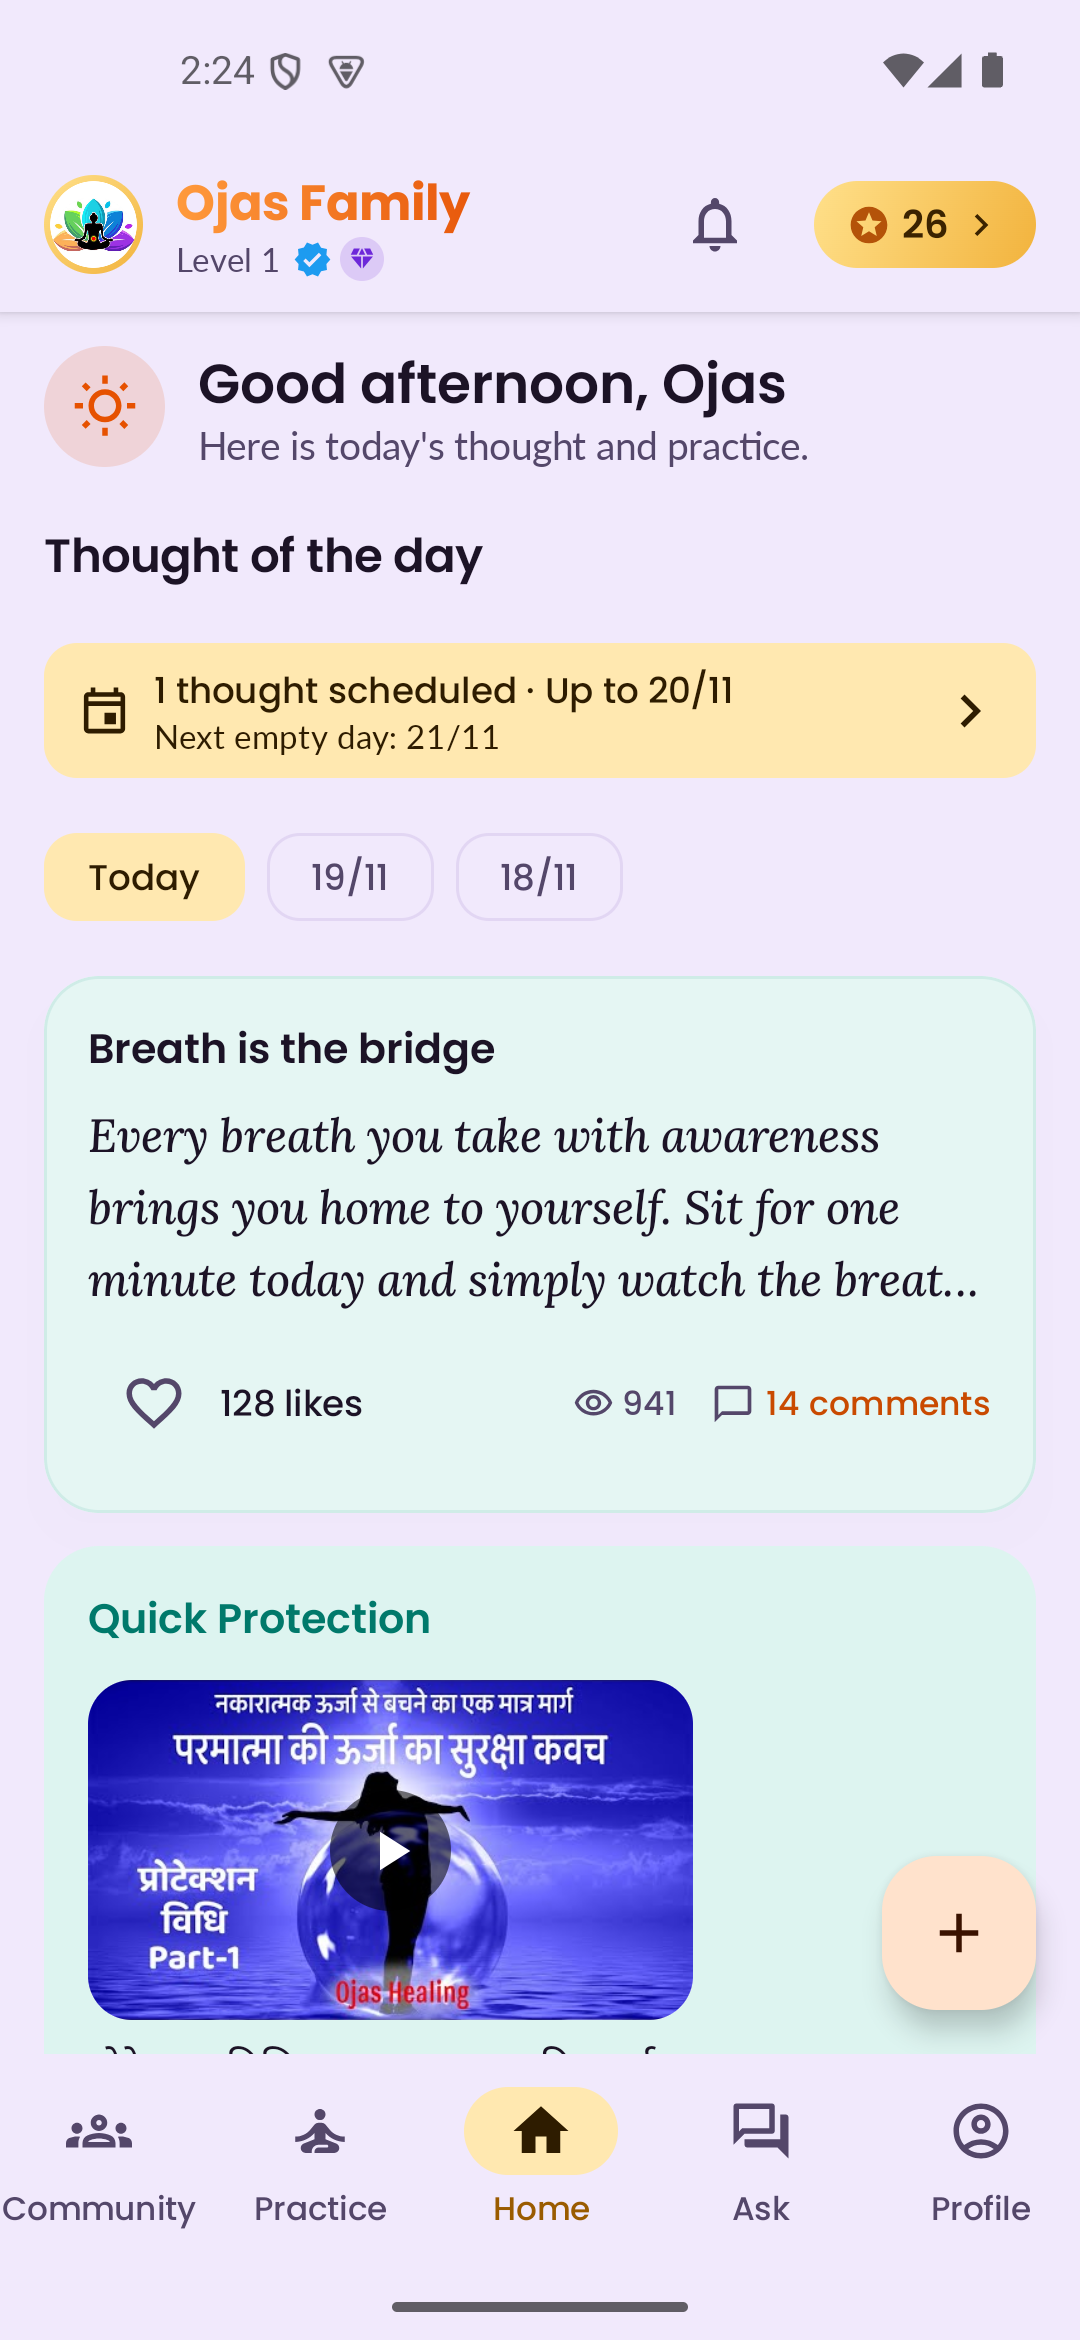
\includegraphics[height=8.2cm]{images/05-home.png}};
\end{tikzpicture}
\vspace*{12.3cm}

{\renewcommand{\arraystretch}{1.25}
\begin{tabularx}{\textwidth}{@{}p{3.6cm}L@{}}
\textcolor{ojDeep}{\bfseries Document} & Ojas Family \textendash\ Solution Architecture \\
\textcolor{ojDeep}{\bfseries Version} & 2.0 (Silver and Gold plans, paid chat and calls) \\
\textcolor{ojDeep}{\bfseries Date} & 20 November 2026 \\
\textcolor{ojDeep}{\bfseries System} & \texttt{com.ojashealing.family} (Android), Firebase project \texttt{ojas-family-app} \\
\textcolor{ojDeep}{\bfseries Region} & asia-south1 (Mumbai) \\
\textcolor{ojDeep}{\bfseries Classification} & Internal \textendash\ engineering and product \\
\end{tabularx}}

\vspace{0.9cm}
\noindent\kpi{73}{Cloud Functions}{ojLav}\hfill
\kpi{38}{Firestore collections}{ojGoldL}\hfill
\kpi{608}{automated tests}{ojTealL}\hfill
\kpi{3}{languages}{ojRose}
\end{titlepage}

% ================= DOCUMENT CONTROL =================
\pagenumbering{roman}
\chapter*{Document control}
\addcontentsline{toc}{chapter}{Document control}
\markboth{Document control}{}

\section*{Revision history}
\begin{tabularx}{\textwidth}{@{}p{1.6cm}p{2.6cm}L@{}}
\headrow \thead{Version} & \thead{Date} & \thead{Change} \\
1.0 & 12 Nov 2026 & Level-based access (User Level 1\textendash4, Member Level 1\textendash3), Ask Swamiji AI, points. \\
1.5 & 19 Nov 2026 & Audio-only guided practices, books with read aloud, YouTube link previews; point gifts removed. \\
\rowcolor{ojLav} 2.0 & 20 Nov 2026 & Free / Silver / Gold plan table replaces level gates; Moderator role; Gold subscription and upgrade; paid chat and calls with the team (day 1) or Swamiji (6 months). \\
\bottomrule
\end{tabularx}

\section*{Audience}
Product owner, administrators, Android and backend engineers, and anyone reviewing security, cost or operations. Each chapter opens with a short summary so non-engineers can read the first paragraph and move on.

\section*{How to read the diagrams}
\begin{center}
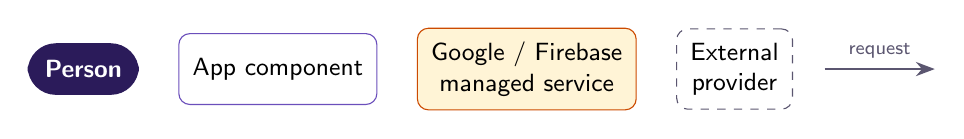
\begin{tikzpicture}[node distance=0.5cm]
  \node[actor] (a) {Person};
  \node[box,right=of a] (b) {App component};
  \node[svc,right=of b] (c) {Google / Firebase\\managed service};
  \node[ext,right=of c] (d) {External\\provider};
  \draw[flow] ($(d.east)+(0.4,0)$) -- node[lbl,above=2pt]{request} ++(1.4,0);
\end{tikzpicture}
\end{center}

\tableofcontents
\listoffigures
\listoftables

\clearpage
\pagenumbering{arabic}

% =====================================================================
\chapter{Executive summary}
\label{chap:exec}

Ojas Family is the community app of Ojas Healing (Swami Anand Swaroop). Members read a daily \emph{Thought of the Day}, practise guided audio meditations, watch and read Swamiji's teachings, ask questions to the community and to an AI trained on Swamiji's teachings, and \textendash\ for a fee \textendash\ chat or call one-to-one with the team or with Swamiji.

The solution is \textbf{serverless}: a native Android app (Kotlin, Jetpack Compose) talks directly to Google Firebase (Authentication, Cloud Firestore, Cloud Storage, Cloud Messaging) under strict security rules, and to 73 Cloud Functions in Mumbai (asia-south1) for everything that must be trusted: payments, points, AI, statistics and notifications. A small admin website on Firebase Hosting gives the owner and administrators their tools.

\begin{center}
\kpi{28.4k}{lines of Kotlin}{ojLav}\hfill
\kpi{4.1k}{lines of TypeScript}{ojGoldL}\hfill
\kpi{874}{lines of security rules}{ojTealL}\hfill
\kpi{EN\,·\,HI\,·\,GU}{interface languages}{ojRose}
\end{center}

\begin{keybox}[Architecture at a glance]
\begin{itemize}
  \item \textbf{Client}: Android 7.0+ (minSdk 24, targetSdk 36), Jetpack Compose, MVVM with hand-written dependency injection, offline Firestore cache, Media3 audio and video.
  \item \textbf{Backend}: Firebase Auth (Google, phone, email), Firestore (38 collections), Storage, FCM, App Check (Play Integrity), 73 Cloud Functions (Node 22, TypeScript).
  \item \textbf{Payments}: Google Play Billing 8 (Silver and Gold subscriptions, chat and call packs), verified server-side with the Play Developer API and real-time notifications.
  \item \textbf{AI}: Ask Swamiji AI \textendash\ retrieval over Swamiji's teachings with NVIDIA embeddings and a hosted NVIDIA large model, streamed to the app.
  \item \textbf{Calls}: WebRTC audio and video, Firestore signalling, Cloudflare TURN relays.
  \item \textbf{Access}: one plan table (Free, Silver Rs.\,49, Gold Rs.\,101 per month) mirrored in the app, the functions and the security rules.
\end{itemize}
\end{keybox}

\section{Key architecture decisions}
\begin{tabularx}{\textwidth}{@{}p{4.3cm}L@{}}
\headrow \thead{Decision} & \thead{Reason} \\
Serverless Firebase & No servers to patch; scales from tens to tens of thousands of members; pay per use. \\
Rules as the security boundary & The app writes directly to Firestore; rules decide every read and write, so a modified app gains nothing. \\
Functions for trusted work & Payments, points, limits, AI keys and counters are never computed on the phone. \\
One plan table in three places & \texttt{PlanAccess.kt}, \texttt{access.ts} and \texttt{allowed(u,s,g)} in the rules hold the same numbers; tests pin all three. \\
NVIDIA hosted AI & Chosen by the owner over Vertex AI / on-device models; the API key stays in Secret Manager. \\
Audio-only guided practice & Smaller downloads, works on slow networks, plays with the screen off. \\
Region asia-south1 & Members are mostly in India; lowest latency and data stays in-country. \\
\bottomrule
\end{tabularx}

% =====================================================================
\chapter{Business context and requirements}

\section{Stakeholders and roles}
\begin{tabularx}{\textwidth}{@{}p{3cm}L@{}}
\headrow \thead{Role} & \thead{What they do in the system} \\
Member (Free) & Reads, practises, asks; features open with time since joining. \\
Silver / Gold member & Paid plan (Rs.\,49 / Rs.\,101 a month): features open sooner, more AI questions. \\
Moderator & Answers chats Swamiji assigns; follows their own plan for everything else. \\
Swamiji & Full access; posts announcements, answers questions, chats and calls. \\
Admin & Full access plus the admin website: members, access grants, content, statistics. \\
\bottomrule
\end{tabularx}

\section{Functional capabilities}
\begin{figure}[H]
\centering
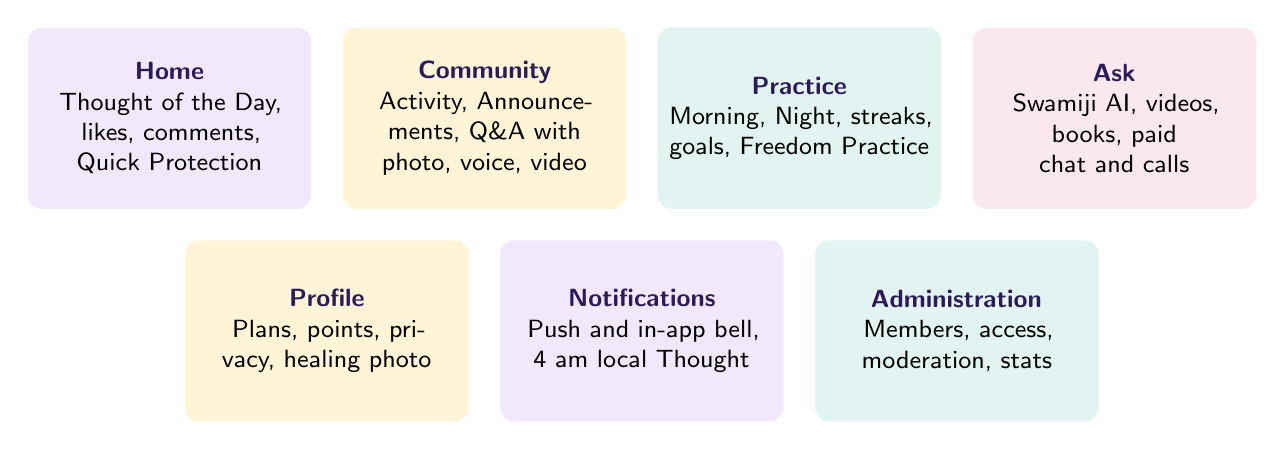
\begin{tikzpicture}[
  cap/.style={draw=none,fill=#1,rounded corners=5pt,minimum width=3.6cm,minimum height=2.3cm,align=center,font=\small,text width=3.3cm},
  ttl/.style={font=\bfseries\small,text=ojDeep}]
  \node[cap=ojLav] (h) at (0,0) {{\bfseries\color{ojDeep}Home}\\Thought of the Day, likes, comments, Quick Protection};
  \node[cap=ojGoldL] (c) at (4,0) {{\bfseries\color{ojDeep}Community}\\Activity, Announcements, Q\&A with photo, voice, video};
  \node[cap=ojTealL] (p) at (8,0) {{\bfseries\color{ojDeep}Practice}\\Morning, Night, streaks, goals, Freedom Practice};
  \node[cap=ojRose] (a) at (12,0) {{\bfseries\color{ojDeep}Ask}\\Swamiji AI, videos, books, paid chat and calls};
  \node[cap=ojGoldL] (pr) at (2,-2.7) {{\bfseries\color{ojDeep}Profile}\\Plans, points, privacy, healing photo};
  \node[cap=ojLav] (n) at (6,-2.7) {{\bfseries\color{ojDeep}Notifications}\\Push and in-app bell, 4 am local Thought};
  \node[cap=ojTealL] (ad) at (10,-2.7) {{\bfseries\color{ojDeep}Administration}\\Members, access, moderation, stats};
\end{tikzpicture}
\caption{Functional capability map}
\end{figure}

\section{Non-functional requirements}
\begin{tabularx}{\textwidth}{@{}p{3.1cm}L p{3.6cm}@{}}
\headrow \thead{Quality} & \thead{Requirement} & \thead{How it is met} \\
Availability & App usable on poor networks; reading works offline. & Firestore offline cache, media cache, retries. \\
Performance & Home opens in under 2 s on mid-range phones. & Paged queries, Compose lazy lists, image sizing. \\
Security & No client can grant itself access, points or payments. & Rules + Functions + App Check. \\
Privacy & Date of birth never shown; profiles can be hidden. & Public profile mirror, field-level rules. \\
Scalability & 10k+ members without redesign. & Serverless, counters via triggers, max 10 instances per function. \\
Localisation & English, Hindi, Gujarati. & Three hand-edited string files. \\
Cost & Stay inside free tiers at today's size. & Cached config, bounded queries, scheduled sweeps. \\
\bottomrule
\end{tabularx}

% =====================================================================
\chapter{Solution overview}

\section{System context}
The diagram shows who uses the system and which outside services it depends on.

\begin{figure}[H]
\centering
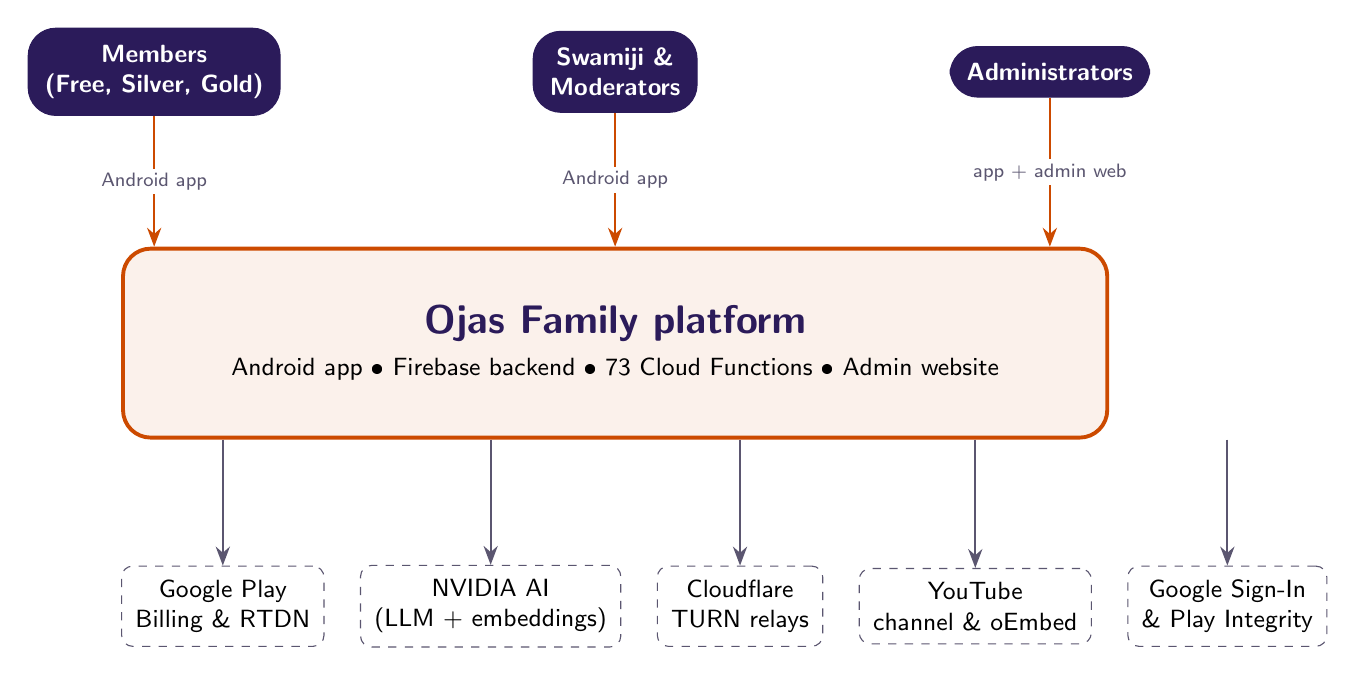
\begin{tikzpicture}[node distance=1.1cm and 1.4cm]
  \node[actor] (mem) {Members\\(Free, Silver, Gold)};
  \node[actor,right=3.2cm of mem] (sw) {Swamiji \&\\Moderators};
  \node[actor,right=3.2cm of sw] (adm) {Administrators};

  \node[draw=ojOrange,fill=ojOrange!8,line width=1.4pt,rounded corners=10pt,minimum width=12.5cm,minimum height=2.4cm,align=center,below=1.7cm of sw] (sys)
    {{\bfseries\Large\color{ojDeep} Ojas Family platform}\\[3pt]\small Android app \textbullet\ Firebase backend \textbullet\ 73 Cloud Functions \textbullet\ Admin website};

  \draw[flowO] (mem) -- node[lbl]{Android app} (mem|-sys.north);
  \draw[flowO] (sw) -- node[lbl]{Android app} (sys.north);
  \draw[flowO] (adm) -- node[lbl]{app + admin web} (adm|-sys.north);

  \node[ext,below=1.6cm of sys.south west,anchor=north west] (play) {Google Play\\Billing \& RTDN};
  \node[ext,right=0.45cm of play] (nv) {NVIDIA AI\\(LLM + embeddings)};
  \node[ext,right=0.45cm of nv] (cf) {Cloudflare\\TURN relays};
  \node[ext,right=0.45cm of cf] (yt) {YouTube\\channel \& oEmbed};
  \node[ext,right=0.45cm of yt] (gg) {Google Sign-In\\\& Play Integrity};
  \foreach \n in {play,nv,cf,yt,gg} \draw[flow] (sys.south -| \n) -- (\n);
\end{tikzpicture}
\caption{System context (C4 level 1)}
\label{fig:context}
\end{figure}

\section{Container view}
\begin{figure}[H]
\centering
\resizebox{\textwidth}{!}{%
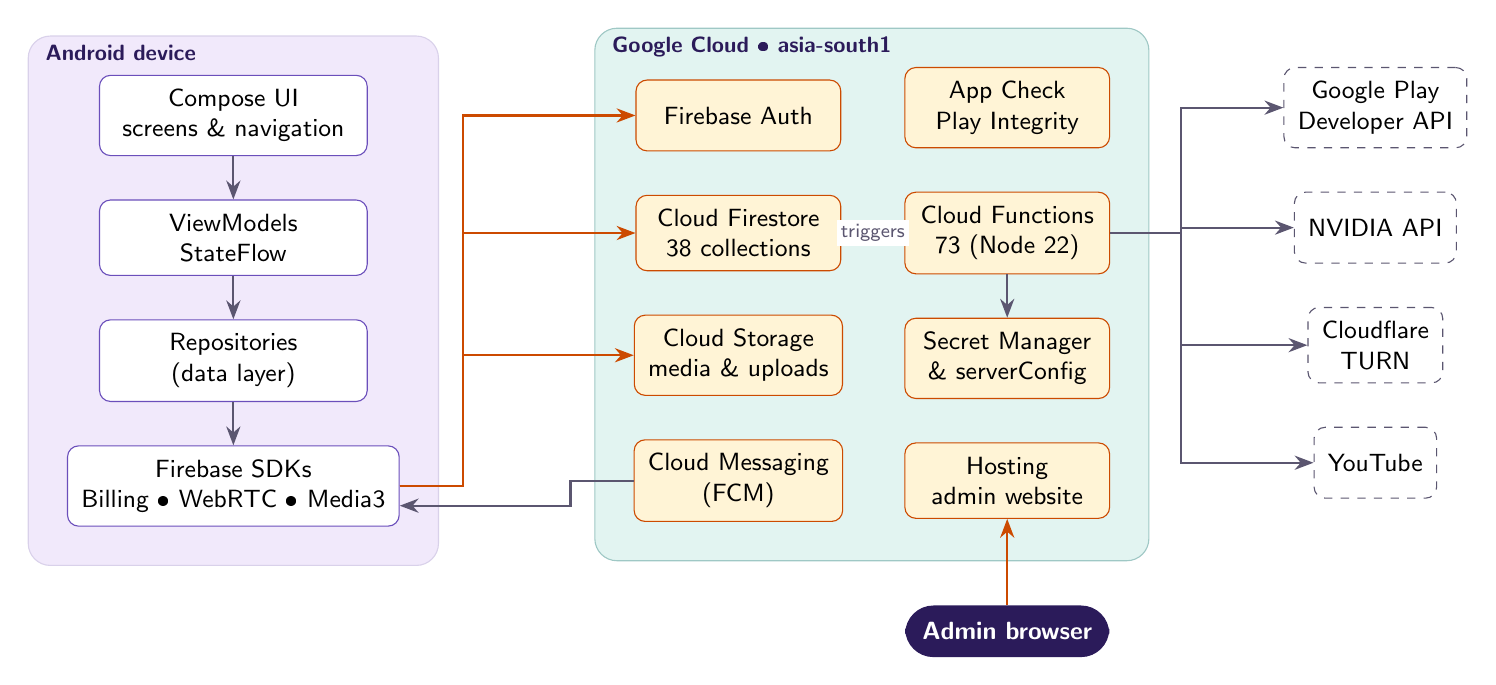
\begin{tikzpicture}[node distance=0.55cm]
  % Device zone
  \node[box,minimum width=3.4cm] (ui) {Compose UI\\screens \& navigation};
  \node[box,below=of ui,minimum width=3.4cm] (vm) {ViewModels\\StateFlow};
  \node[box,below=of vm,minimum width=3.4cm] (repo) {Repositories\\(data layer)};
  \node[box,below=of repo,minimum width=3.4cm] (sdk) {Firebase SDKs\\Billing \textbullet\ WebRTC \textbullet\ Media3};
  \draw[flow] (ui) -- (vm); \draw[flow] (vm) -- (repo); \draw[flow] (repo) -- (sdk);
  \begin{scope}[on background layer]
    \node[zone,fit=(ui)(sdk),inner sep=14pt] (dev) {};
  \end{scope}
  \node[zlabel] at (dev.north west) {\ Android device};

  % Firebase zone
  \node[svc,right=3.4cm of ui] (auth) {Firebase Auth};
  \node[svc,below=of auth] (fs) {Cloud Firestore\\38 collections};
  \node[svc,below=of fs] (st) {Cloud Storage\\media \& uploads};
  \node[svc,below=of st] (fcm) {Cloud Messaging\\(FCM)};
  \node[svc,right=0.8cm of fs] (fn) {Cloud Functions\\73 (Node 22)};
  \node[svc,above=of fn] (ac) {App Check\\Play Integrity};
  \node[svc,below=of fn] (sec) {Secret Manager\\\& serverConfig};
  \node[svc,below=of sec] (host) {Hosting\\admin website};
  \begin{scope}[on background layer]
    \node[zoneT,fit=(auth)(fcm)(fn)(host)(ac),inner sep=14pt] (fb) {};
  \end{scope}
  \node[zlabel] at (fb.north west) {\ Google Cloud \textbullet\ asia-south1};

  \draw[flowO] (sdk.east) -- ++(0.8,0) |- (auth.west);
  \draw[flowO] (sdk.east) -- ++(0.8,0) |- (fs.west);
  \draw[flowO] (sdk.east) -- ++(0.8,0) |- (st.west);
  \draw[flow] (fcm.west) -- ++(-0.8,0) |- ($(sdk.east)+(0,-0.25)$);
  \draw[flow] (fs) -- node[lbl]{triggers} (fn);
  \draw[flow] (fn) -- (sec);

  % External
  \node[ext,right=2.2cm of ac] (play) {Google Play\\Developer API};
  \node[ext,below=of play] (nv) {NVIDIA API};
  \node[ext,below=of nv] (cf) {Cloudflare\\TURN};
  \node[ext,below=of cf] (yt) {YouTube};
  \foreach \n in {play,nv,cf,yt} \draw[flow] (fn.east) -- ++(0.9,0) |- (\n.west);

  \node[actor,below=1.1cm of host] (admin) {Admin browser};
  \draw[flowO] (admin) -- (host);
\end{tikzpicture}}
\caption{Container view (C4 level 2)}
\label{fig:containers}
\end{figure}

% =====================================================================
\chapter{Android application architecture}

\section{Layers}
The app follows a unidirectional data flow: Firestore snapshots become Kotlin flows in repositories, ViewModels combine them into immutable UI state, and Compose renders that state. User actions travel back the same way.

\begin{figure}[H]
\centering
\begin{tikzpicture}[layer/.style={draw=none,fill=#1,rounded corners=6pt,minimum width=13.5cm,minimum height=1.25cm,align=left,text width=13cm,font=\small}]
  \node[layer=ojLav] (l1) at (0,0) {\textbf{UI} \textbullet\ \texttt{ui/} \textendash\ Compose screens (home, community, ask, practice, profile, paid, admin), Material 3 theme, adaptive layouts};
  \node[layer=ojGoldL] (l2) at (0,-1.55) {\textbf{State} \textbullet\ ViewModels expose \texttt{StateFlow<Ui>}; \texttt{combine} of profile, entitlements and data flows};
  \node[layer=ojTealL] (l3) at (0,-3.1) {\textbf{Domain} \textbullet\ \texttt{domain/} \textendash\ \texttt{PlanAccess}, \texttt{Permissions}, \texttt{Content}, roles and levels (pure Kotlin, unit tested)};
  \node[layer=ojRose] (l4) at (0,-4.65) {\textbf{Data} \textbullet\ \texttt{data/} \textendash\ 21 repositories: auth, social, chat, call, paid, ai, books, practice, points, presence\ldots};
  \node[layer=ojLav] (l5) at (0,-6.2) {\textbf{Platform} \textbullet\ Firebase SDKs, Play Billing 8, WebRTC, Media3, Coil, DataStore, WorkManager};
  \foreach \a/\b in {l1/l2,l2/l3,l3/l4,l4/l5} \draw[flowO] ($(\a.south)+(-3,0)$) -- ($(\b.north)+(-3,0)$);
  \foreach \a/\b in {l5/l4,l4/l3,l3/l2,l2/l1} \draw[flow] ($(\a.north)+(3,0)$) -- ($(\b.south)+(3,0)$);
  \node[font=\scriptsize,text=ojOrange] at (-4.4,-0.78) {actions};
  \node[font=\scriptsize,text=ojGrey] at (4.3,-0.78) {state};
\end{tikzpicture}
\caption{Android layers and data flow}
\end{figure}

\section{Technology stack}
\begin{tabularx}{\textwidth}{@{}p{3.6cm}p{3.2cm}L@{}}
\headrow \thead{Area} & \thead{Choice} & \thead{Notes} \\
Language & Kotlin 2.2 & Coroutines 1.10, kotlinx.serialization 1.9 \\
UI & Jetpack Compose (BOM 2025.08) & Material 3, material3-adaptive, type-safe navigation \\
Build & AGP 9.1, Gradle 9.3 & compileSdk 37, targetSdk 36, minSdk 24; ABI splits \\
Backend SDK & Firebase BOM 34.17 & Auth, Firestore, Storage, Functions, Messaging, App Check, Crashlytics, Analytics \\
Payments & Play Billing 8.0 & Subscriptions, one-time packs, subscription replacement \\
Media & Media3 1.8 & ExoPlayer for practice audio and video \\
Images & Coil 2.7 & Cached, sized thumbnails \\
Calls & WebRTC & Peer-to-peer with TURN fallback \\
DI & Hand-written \texttt{AppContainer} & No annotation processing; fast builds \\
\bottomrule
\end{tabularx}

\section{Local development backend}
Debug builds can switch to the Firebase emulators with one property (\texttt{debug.ojas.emulator}); the project id becomes \texttt{demo-ojas}, which the emulators treat as local only, so no push, payment or data reaches production. The screenshots in Chapter~\ref{chap:screens} were taken this way with sample data.

% =====================================================================
\chapter{Backend architecture}

\section{Cloud Functions inventory}
Seventy-three functions run in asia-south1 with at most ten instances each. Most are small event handlers that keep counters, notifications and statistics in step.

\begin{figure}[H]
\centering
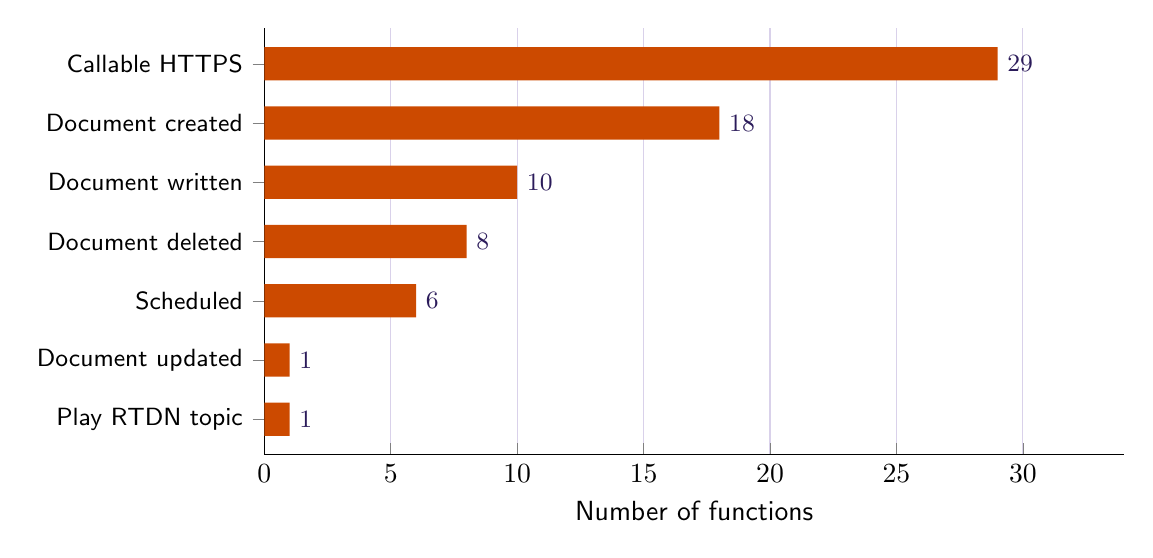
\begin{tikzpicture}
\begin{axis}[
  xbar, width=12.5cm, height=7cm, bar width=12pt,
  xmin=0, xmax=34, xlabel={Number of functions},
  symbolic y coords={Play RTDN topic,Document updated,Scheduled,Document deleted,Document written,Document created,Callable HTTPS},
  ytick=data, y tick label style={font=\small},
  nodes near coords, nodes near coords style={font=\small\bfseries,color=ojDeep},
  axis x line*=bottom, axis y line*=left, major grid style={ojLine}, xmajorgrids,
  ]
\addplot[fill=ojOrange,draw=none] coordinates {(1,Play RTDN topic) (1,Document updated) (6,Scheduled) (8,Document deleted) (10,Document written) (18,Document created) (29,Callable HTTPS)};
\end{axis}
\end{tikzpicture}
\caption{Cloud Functions by trigger type (73 in total)}
\label{fig:fncount}
\end{figure}

\begin{tabularx}{\textwidth}{@{}p{3.3cm}L@{}}
\headrow \thead{Domain} & \thead{Functions (examples)} \\
Membership \& billing & \texttt{verifyPurchase}, \texttt{playNotification}, \texttt{adminGrant}, \texttt{paidDayTick} \\
Access \& roles & \texttt{setRole}, \texttt{syncRole}, \texttt{adminApplyAdminList}, \texttt{deleteAccount} \\
AI & \texttt{askSwamiji} (streaming), \texttt{aiQuota}, \texttt{rateAiAnswer} \\
Community & \texttt{questionWritten} (daily Q\&A limit), \texttt{answerWritten}, like/view counters (26) \\
Practice \& points & \texttt{startPractice}, \texttt{completePractice}, \texttt{logPractice}, \texttt{claimDailyOpen}, \texttt{tickGoal} \\
Chat \& calls & \texttt{chatMessageCreated}, \texttt{callCreated}, \texttt{callUpdated}, \texttt{turnCredentials}, \texttt{sweepCalls} \\
Content & \texttt{addVideo}, \texttt{importPlaylist}, \texttt{linkPreview} \\
Admin \& stats & \texttt{adminStats}, \texttt{adminDayStats}, \texttt{dailyStats}, \texttt{userCounts} \\
\bottomrule
\end{tabularx}

\section{Scheduled jobs}
\begin{tabularx}{\textwidth}{@{}p{3.4cm}p{3.6cm}L@{}}
\headrow \thead{Job} & \thead{Schedule} & \thead{Purpose} \\
\texttt{thoughtOfDayPush} & every 15 min (UTC) & Sends the Thought at 4 am in each member's time zone. \\
\texttt{paidDayTick} & 00:05 IST daily & Counts a paid day for every active member; refreshes plan fields. \\
\texttt{dailyStats} & 00:20 IST daily & Builds yesterday's usage statistics for the admin site. \\
\texttt{bellSweep} & 03:30 IST daily & Trims old in-app notifications. \\
\texttt{callReminders} & every 5 min & Reminds both sides 15 minutes before a scheduled call. \\
\texttt{sweepCalls} & every minute & Marks calls that rang too long as missed. \\
\bottomrule
\end{tabularx}

% =====================================================================
\chapter{Data architecture}

\section{Firestore collections by domain}
\begin{figure}[H]
\centering
\resizebox{\textwidth}{!}{%
\begin{tikzpicture}[
  grp/.style={draw=none,fill=#1,rounded corners=6pt,inner sep=6pt,text width=3.5cm,align=left,font=\footnotesize},
  gt/.style={font=\small\bfseries,text=ojDeep}]
  \node[grp=ojLav] (u) at (0,0) {\textcolor{ojDeep}{\bfseries People}\\[2pt]\texttt{users/\{uid\}}\\ \quad\texttt{entitlements/}\\ \quad\texttt{counters/}\\ \quad\texttt{chatPrefs/}\\ \quad\texttt{notifications/}\\ \texttt{publicProfiles/}\\ \texttt{presence/}\\ \texttt{facePhotos/}};
  \node[grp=ojGoldL] (c) at (4.4,0) {\textcolor{ojDeep}{\bfseries Community}\\[2pt]\texttt{thoughts/\{day\}}\\ \texttt{announcements/}\\ \texttt{questions/} \texttt{answers/}\\ \texttt{dailyPosts/} \texttt{replies/}\\ \texttt{comments/} \texttt{likes/}\\ \texttt{views/} \texttt{reports/}\\ \texttt{broadcasts/}\\ \texttt{paidBroadcasts/}};
  \node[grp=ojTealL] (k) at (8.8,0) {\textcolor{ojDeep}{\bfseries Content \& practice}\\[2pt]\texttt{content/} (videos)\\ \texttt{books/} \texttt{readQa/}\\ \texttt{goals/} \texttt{practiceLog/}\\ \texttt{knowledge/}\\ \texttt{knowledgeSources/}\\ \texttt{aiChats/} \texttt{aiFeedback/}};
  \node[grp=ojRose] (p) at (13.2,0) {\textcolor{ojDeep}{\bfseries Paid contact}\\[2pt]\texttt{chats/} (Swamiji)\\ \texttt{adminChats/} (team)\\ \quad\texttt{messages/}\\ \texttt{callRequests/}\\ \texttt{calls/}\\ \quad\texttt{candidates/}\\ \texttt{purchases/}};
  \node[grp=ojLav,text width=16.6cm] (o) at (6.6,-3.9) {\textcolor{ojDeep}{\bfseries Operations}\quad \texttt{config/} \textbullet\ \texttt{stats/} \textbullet\ \texttt{pointEvents/} \textbullet\ \texttt{pointAdjustments/} \textbullet\ \texttt{pointTransfers/} (read-only history) \textbullet\ \texttt{serverConfig/} (functions only)};
\end{tikzpicture}}
\caption{Firestore collections grouped by domain}
\end{figure}

\section{The member record and entitlements}
\begin{figure}[H]
\centering
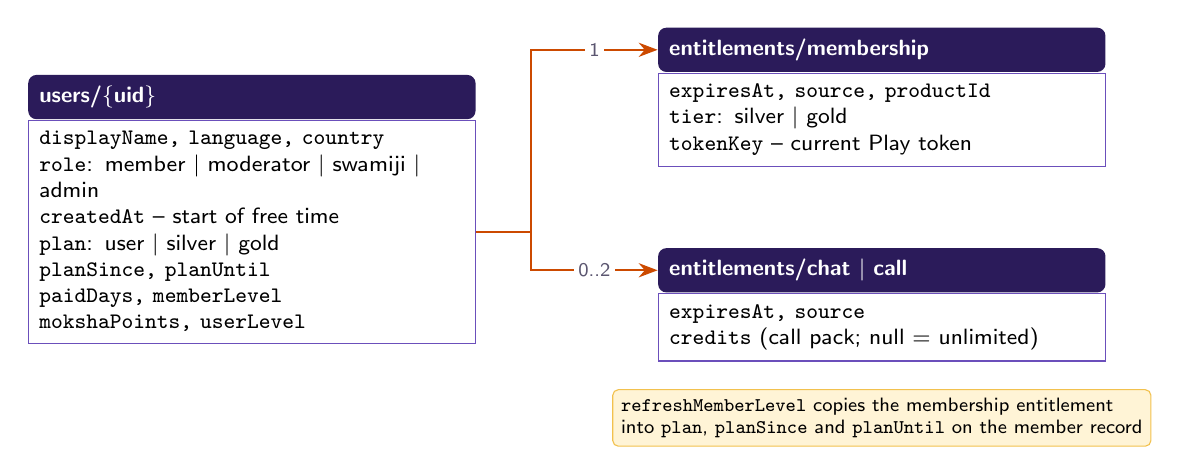
\begin{tikzpicture}[
  eh/.style={fill=ojDeep,text=white,font=\footnotesize\bfseries,text width=5.4cm,inner sep=4pt,rounded corners=3pt},
  eb/.style={draw=ojPurple,fill=white,font=\footnotesize,text width=5.4cm,align=left,inner sep=4pt}]
  \node[eh] (uh) at (0,0) {users/\{uid\}};
  \node[eb,below=0pt of uh] (u) {\texttt{displayName, language, country}\\\texttt{role}: member \textbar\ moderator \textbar\ swamiji \textbar\ admin\\\texttt{createdAt} \textendash\ start of free time\\\texttt{plan}: user \textbar\ silver \textbar\ gold\\\texttt{planSince, planUntil}\\\texttt{paidDays, memberLevel}\\\texttt{mokshaPoints, userLevel}};
  \node[eh] (eh1) at (8,0.6) {entitlements/membership};
  \node[eb,below=0pt of eh1] (e) {\texttt{expiresAt, source, productId}\\\texttt{tier}: silver \textbar\ gold\\\texttt{tokenKey} \textendash\ current Play token};
  \node[eh] (eh2) at (8,-2.2) {entitlements/chat \textbar\ call};
  \node[eb,below=0pt of eh2] (c) {\texttt{expiresAt, source}\\\texttt{credits} (call pack; null = unlimited)};
  \draw[flowO] (u.east) -- ++(0.7,0) |- node[lbl,pos=0.75]{1} (eh1.west);
  \draw[flowO] (u.east) -- ++(0.7,0) |- node[lbl,pos=0.75]{0..2} (eh2.west);
  \node[note,anchor=north] at ($(c.south)+(0,-0.35)$) {\texttt{refreshMemberLevel} copies the membership entitlement\\into \texttt{plan}, \texttt{planSince} and \texttt{planUntil} on the member record};
\end{tikzpicture}
\caption{Member record and paid access (written only by Cloud Functions)}
\end{figure}

\begin{notebox}[Who may write what]
Members can edit their own profile fields, but \texttt{role}, \texttt{plan}, \texttt{planSince}, \texttt{planUntil}, points and every \texttt{entitlements/} document are written only by Cloud Functions. The rules reject any client write to them.
\end{notebox}

% =====================================================================
\chapter{Membership and access model}

\section{Plans}
\begin{center}
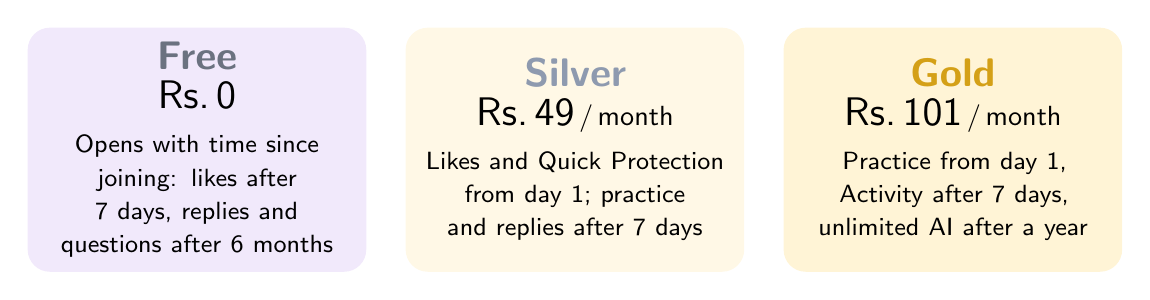
\begin{tikzpicture}[plan/.style={draw=none,fill=#1,rounded corners=8pt,minimum width=4.3cm,minimum height=3.1cm,align=center,text width=3.9cm}]
  \node[plan=ojLav] at (0,0) {{\color{free}\bfseries\Large Free}\\[2pt]{\Large Rs.\,0}\\[4pt]\small Opens with time since joining: likes after 7 days, replies and questions after 6 months};
  \node[plan=ojGoldL!60!white] at (4.8,0) {{\color{silver}\bfseries\Large Silver}\\[2pt]{\Large Rs.\,49}\,/\,month\\[4pt]\small Likes and Quick Protection from day 1; practice and replies after 7 days};
  \node[plan=ojGoldL] at (9.6,0) {{\color{gold}\bfseries\Large Gold}\\[2pt]{\Large Rs.\,101}\,/\,month\\[4pt]\small Practice from day 1, Activity after 7 days, unlimited AI after a year};
\end{tikzpicture}
\end{center}

A member's \emph{stage} counts from \texttt{createdAt} on the free plan, or from \texttt{planSince} while a paid plan runs; the member gets whichever opens a feature sooner. Swamiji and admins have everything; moderators follow their own plan.

\section{The access table}
\newcommand{\cellF}[1]{\cellcolor{ojTealL}#1}
\newcommand{\cellN}{\cellcolor{ojRose}\textcolor{ojOrange}{never}}
\begin{table}[H]
\centering
\small
\begin{tabular}{@{}lccc@{}}
\headrow \thead{Feature} & \thead{Free} & \thead{Silver} & \thead{Gold} \\
Like posts & 7 days & \cellF{day 1} & \cellF{day 1} \\
Reply on Thought / Q\&A, ask a question & 6 months & 7 days & 7 days \\
Quick Protection practice & 6 months & \cellF{day 1} & \cellF{day 1} \\
Reply on Announcements & 6 months & 7 days & \cellF{day 1} \\
Question with photo, voice or video & 12 months & 12 months & 6 months \\
Read and like Daily Activity & \cellN & 6 months & 7 days \\
Reply on Daily Activity & \cellN & 12 months & 6 months \\
Post Daily Activity & \cellN & \cellN & 12 months \\
Morning and Night practice & \cellN & 7 days & \cellF{day 1} \\
Healing photo & \cellN & 12 months & 6 months \\
Hide profile & \cellN & \cellN & 12 months \\
\rowcolor{ojLav} Paid chat / call with the team & \multicolumn{3}{c}{day 1 (chat or call pack bought separately)} \\
\rowcolor{ojLav} Paid chat / call with Swamiji & \multicolumn{3}{c}{6 months (chat or call pack bought separately)} \\
\bottomrule
\end{tabular}
\caption{What each plan opens, and when (owner's table, 20 Nov 2026)}
\label{tab:access}
\end{table}

\section{Feature timeline}
\begin{figure}[H]
\centering
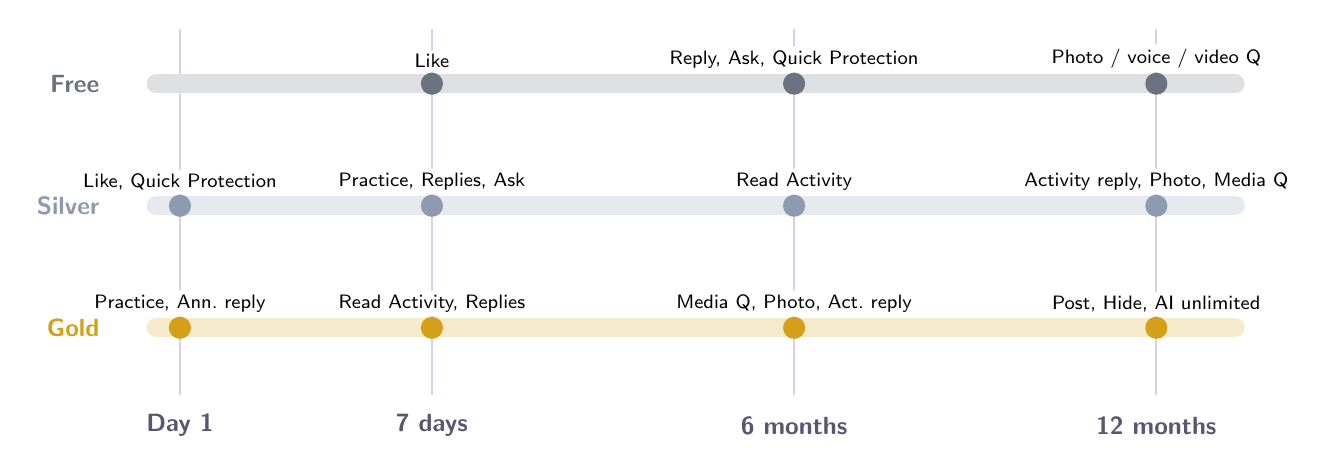
\begin{tikzpicture}[y=1.55cm,
  ev/.style={font=\scriptsize,align=center,fill=white,inner sep=1.5pt,rounded corners=2pt}]
  % Day 1 = 0, 7 days = 3.2, 6 months = 7.8, 12 months = 12.4 (not to scale)
  \foreach \x/\t in {0/Day 1,3.2/7 days,7.8/6 months,12.4/12 months}{
    \draw[ojLine,thick] (\x,-0.55) -- (\x,2.45); \node[font=\small\bfseries,text=ojGrey] at (\x,-0.8) {\t};}
  \foreach \yy/\nm/\col in {0/Gold/gold,1/Silver/silver,2/Free/free}{
    \node[anchor=east,font=\small\bfseries,text=\col] at (-0.9,\yy) {\nm};
    \draw[line width=7pt,\col!22,line cap=round] (-0.3,\yy) -- (13.4,\yy);}
  % Free
  \fill[free] (3.2,2) circle (4pt); \node[ev,above=4pt] at (3.2,2) {Like};
  \fill[free] (7.8,2) circle (4pt); \node[ev,above=4pt] at (7.8,2) {Reply, Ask, Quick Protection};
  \fill[free] (12.4,2) circle (4pt); \node[ev,above=4pt] at (12.4,2) {Photo / voice / video Q};
  % Silver
  \fill[silver] (0,1) circle (4pt); \node[ev,above=4pt] at (0,1) {Like, Quick Protection};
  \fill[silver] (3.2,1) circle (4pt); \node[ev,above=4pt] at (3.2,1) {Practice, Replies, Ask};
  \fill[silver] (7.8,1) circle (4pt); \node[ev,above=4pt] at (7.8,1) {Read Activity};
  \fill[silver] (12.4,1) circle (4pt); \node[ev,above=4pt] at (12.4,1) {Activity reply, Photo, Media Q};
  % Gold
  \fill[gold] (0,0) circle (4pt); \node[ev,above=4pt] at (0,0) {Practice, Ann.\ reply};
  \fill[gold] (3.2,0) circle (4pt); \node[ev,above=4pt] at (3.2,0) {Read Activity, Replies};
  \fill[gold] (7.8,0) circle (4pt); \node[ev,above=4pt] at (7.8,0) {Media Q, Photo, Act.\ reply};
  \fill[gold] (12.4,0) circle (4pt); \node[ev,above=4pt] at (12.4,0) {Post, Hide, AI unlimited};
\end{tikzpicture}
\caption{When features open on each plan}
\end{figure}

\section{Daily limits}
\begin{figure}[H]
\centering
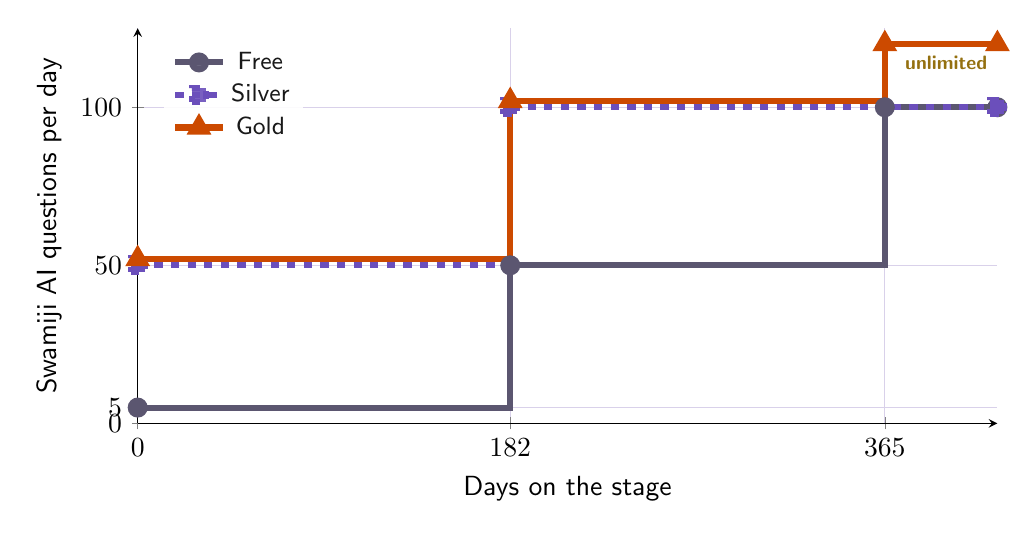
\begin{tikzpicture}
\begin{axis}[
  width=12.5cm,height=6.6cm, xmin=0,xmax=420, ymin=0,ymax=125,
  xlabel={Days on the stage}, ylabel={Swamiji AI questions per day},
  xtick={0,182,365},
  ytick={0,5,50,100}, legend pos=north west, legend style={font=\small,draw=none,fill=white,fill opacity=0.9},
  grid=major, major grid style={ojLine}, axis lines=left, const plot]
\addplot[line width=2.2pt,ojGrey,mark=*,mark size=2.5pt] coordinates {(0,5) (182,50) (365,100) (420,100)}; \addlegendentry{Free}
\addplot[line width=2.2pt,ojPurple,dashed,mark=square*,mark size=2.5pt] coordinates {(0,50) (182,100) (420,100)}; \addlegendentry{Silver}
\addplot[line width=2.2pt,ojOrange,mark=triangle*,mark size=3pt] coordinates {(0,52) (182,102) (365,120) (420,120)}; \addlegendentry{Gold}
\node[font=\scriptsize\bfseries,text=gold!70!black] at (axis cs:395,114) {unlimited};
\end{axis}
\end{tikzpicture}
\caption{Ask Swamiji AI daily limit by plan (Gold is unlimited after a year)}
\end{figure}

\begin{tabularx}{\textwidth}{@{}p{5.4cm}L@{}}
\headrow \thead{Q\&A posts per day} & \thead{Rule} \\
1 & Asking with words only is open (\texttt{AskText}). \\
5 & Photo, voice and video questions are open (\texttt{AskMedia}). \\
10 & Gold after 12 months. \\
\bottomrule
\end{tabularx}
The \texttt{questionWritten} trigger counts posts per member per IST day in \texttt{users/\{uid\}/counters/\{day\}} and removes a question over the limit; the app reads the same counter to warn before posting.

\begin{keybox}[One table, three copies]
\texttt{app/domain/PlanAccess.kt} (what the app shows), \texttt{functions/src/access.ts} (what functions enforce) and \texttt{allowed(u, s, g)} in \texttt{firestore.rules} (what the database allows) hold the same numbers. A change to the table must change all three; the test suites of each layer check it.
\end{keybox}

% =====================================================================
\chapter{Key flows}

\section{Sign-in and onboarding}
\begin{figure}[H]
\centering
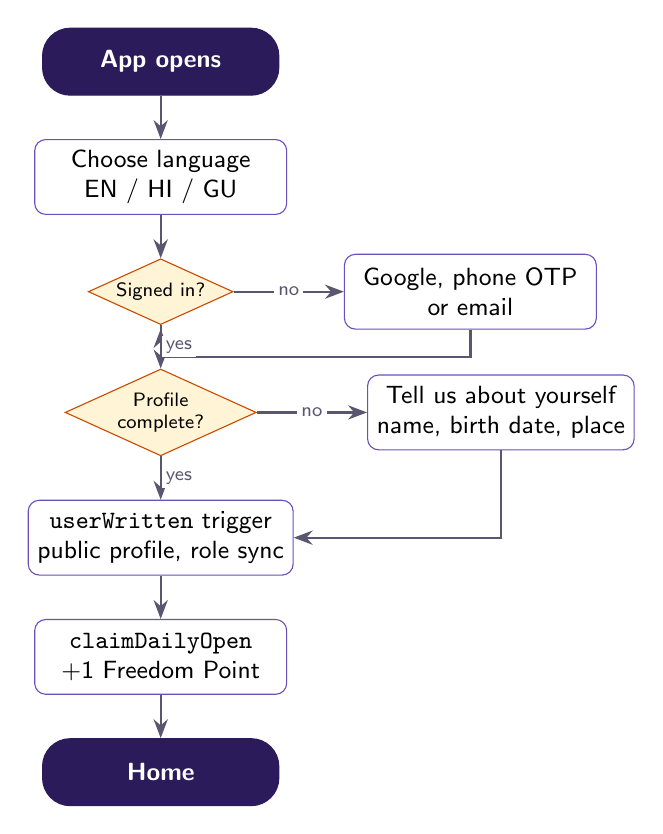
\begin{tikzpicture}[node distance=0.55cm and 0.9cm]
  \node[term] (s) {App opens};
  \node[fstep,below=of s] (lang) {Choose language\\EN / HI / GU};
  \node[dec,below=of lang] (in) {Signed in?};
  \node[fstep,right=1.4cm of in] (auth) {Google, phone OTP\\or email};
  \node[dec,below=of in] (prof) {Profile\\complete?};
  \node[fstep,right=1.4cm of prof] (form) {Tell us about yourself\\name, birth date, place};
  \node[fstep,below=of prof] (fn) {\texttt{userWritten} trigger\\public profile, role sync};
  \node[fstep,below=of fn] (pts) {\texttt{claimDailyOpen}\\+1 Freedom Point};
  \node[term,below=of pts] (home) {Home};
  \draw[flow] (s) -- (lang); \draw[flow] (lang) -- (in);
  \draw[flow] (in) -- node[lbl]{no} (auth); \draw[flow] (auth.south) -- ++(0,-0.35) -| ($(in.south)+(0.0,-0.05)$);
  \draw[flow] (in) -- node[lbl,right]{yes} (prof);
  \draw[flow] (prof) -- node[lbl]{no} (form); \draw[flow] (form.south) |- (fn.east);
  \draw[flow] (prof) -- node[lbl,right]{yes} (fn); \draw[flow] (fn) -- (pts); \draw[flow] (pts) -- (home);
\end{tikzpicture}
\caption{Sign-in and onboarding flow}
\end{figure}

\section{Buying a plan or pack (Google Play)}
\begin{figure}[H]
\centering
\resizebox{\textwidth}{!}{%
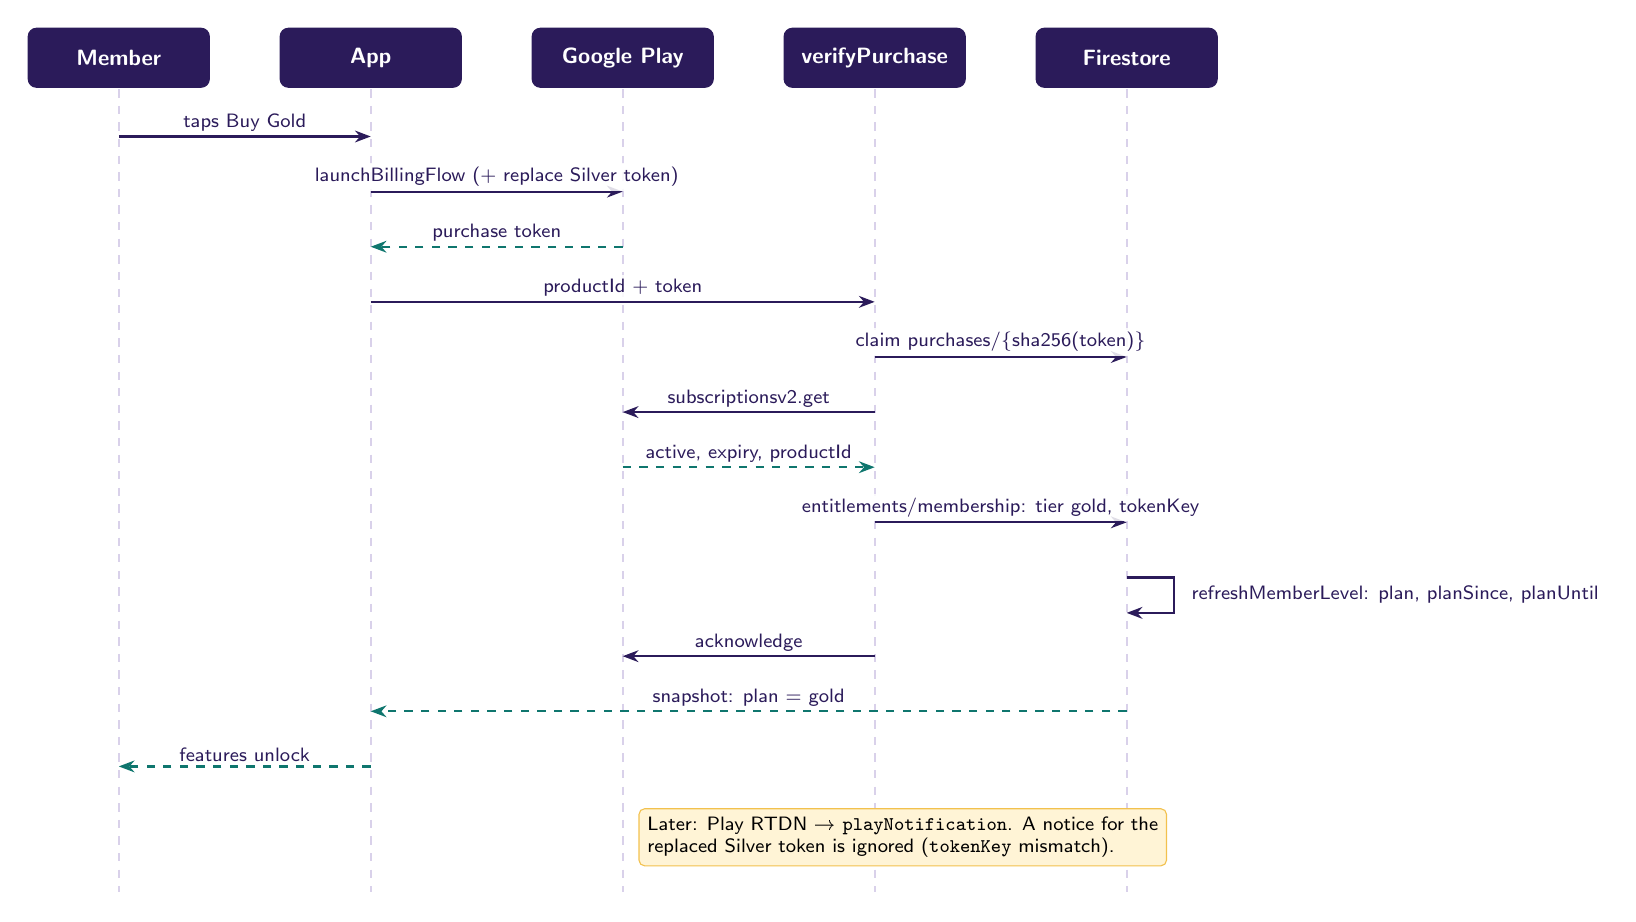
\begin{tikzpicture}
  \foreach \x/\n in {0/Member,3.2/App,6.4/Google Play,9.6/verifyPurchase,12.8/Firestore}{
    \node[part] at (\x,0) {\n}; \draw[life] (\x,-0.4) -- (\x,-10.6);}
  \seqmsg{0}{3.2}{-1.0}{taps Buy Gold}
  \seqmsg{3.2}{6.4}{-1.7}{launchBillingFlow (+ replace Silver token)}
  \seqret{6.4}{3.2}{-2.4}{purchase token}
  \seqmsg{3.2}{9.6}{-3.1}{productId + token}
  \seqmsg{9.6}{12.8}{-3.8}{claim purchases/\{sha256(token)\}}
  \seqmsg{9.6}{6.4}{-4.5}{subscriptionsv2.get}
  \seqret{6.4}{9.6}{-5.2}{active, expiry, productId}
  \seqmsg{9.6}{12.8}{-5.9}{entitlements/membership: tier gold, tokenKey}
  \seqself{12.8}{-6.6}{refreshMemberLevel: plan, planSince, planUntil}
  \seqmsg{9.6}{6.4}{-7.6}{acknowledge}
  \seqret{12.8}{3.2}{-8.3}{snapshot: plan = gold}
  \seqret{3.2}{0}{-9.0}{features unlock}
  \node[note,anchor=west] at (6.6,-9.9) {Later: Play RTDN \textrightarrow\ \texttt{playNotification}. A notice for the\\replaced Silver token is ignored (\texttt{tokenKey} mismatch).};
\end{tikzpicture}}
\caption{Purchase verification sequence, including the Silver-to-Gold upgrade}
\end{figure}

\section{Ask Swamiji AI}
\begin{figure}[H]
\centering
\resizebox{\textwidth}{!}{%
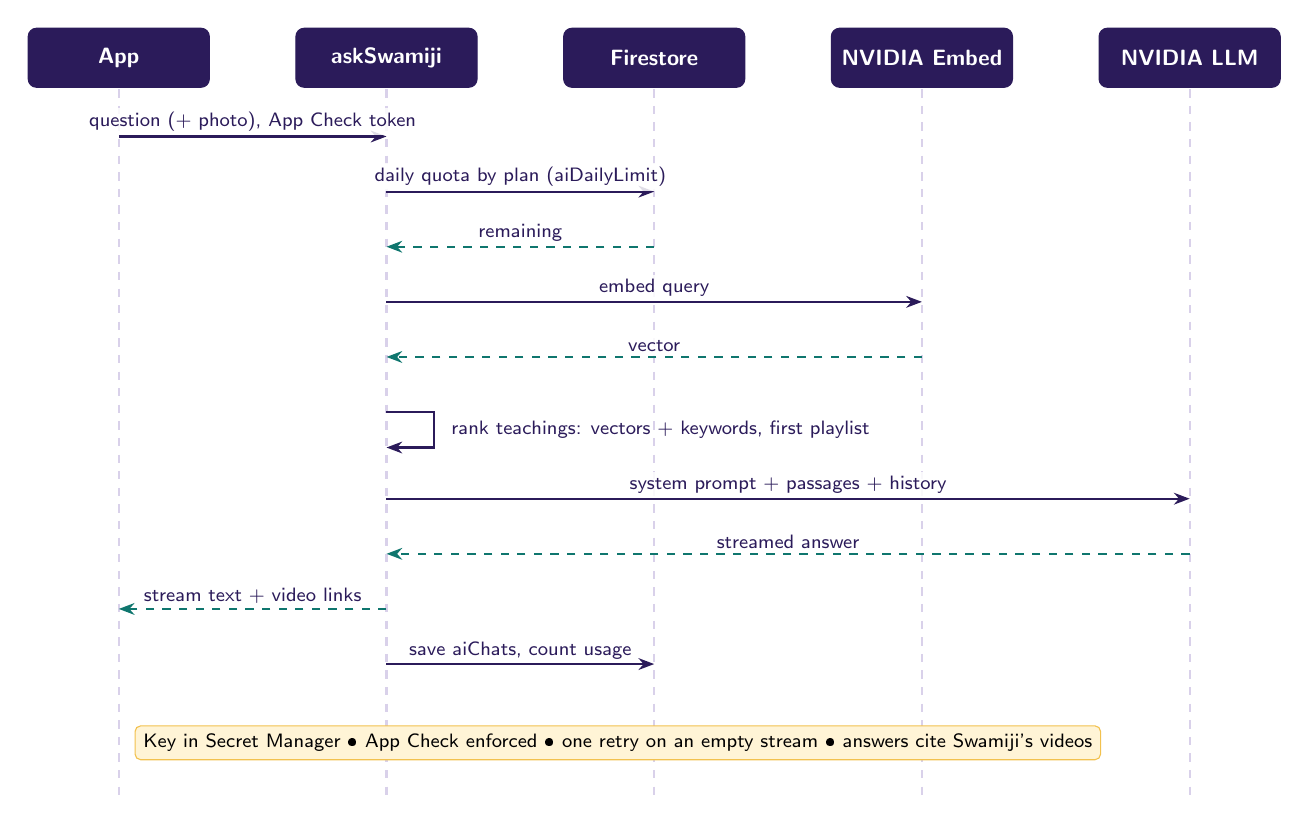
\begin{tikzpicture}
  \foreach \x/\n in {0/App,3.4/askSwamiji,6.8/Firestore,10.2/NVIDIA Embed,13.6/NVIDIA LLM}{
    \node[part] at (\x,0) {\n}; \draw[life] (\x,-0.4) -- (\x,-9.4);}
  \seqmsg{0}{3.4}{-1.0}{question (+ photo), App Check token}
  \seqmsg{3.4}{6.8}{-1.7}{daily quota by plan (aiDailyLimit)}
  \seqret{6.8}{3.4}{-2.4}{remaining}
  \seqmsg{3.4}{10.2}{-3.1}{embed query}
  \seqret{10.2}{3.4}{-3.8}{vector}
  \seqself{3.4}{-4.5}{rank teachings: vectors + keywords, first playlist}
  \seqmsg{3.4}{13.6}{-5.6}{system prompt + passages + history}
  \seqret{13.6}{3.4}{-6.3}{streamed answer}
  \seqret{3.4}{0}{-7.0}{stream text + video links}
  \seqmsg{3.4}{6.8}{-7.7}{save aiChats, count usage}
  \node[note,anchor=west] at (0.2,-8.7) {Key in Secret Manager \textbullet\ App Check enforced \textbullet\ one retry on an empty stream \textbullet\ answers cite Swamiji's videos};
\end{tikzpicture}}
\caption{Retrieval-augmented answer from Swamiji's teachings}
\end{figure}

\section{Posting a question}
\begin{figure}[H]
\centering
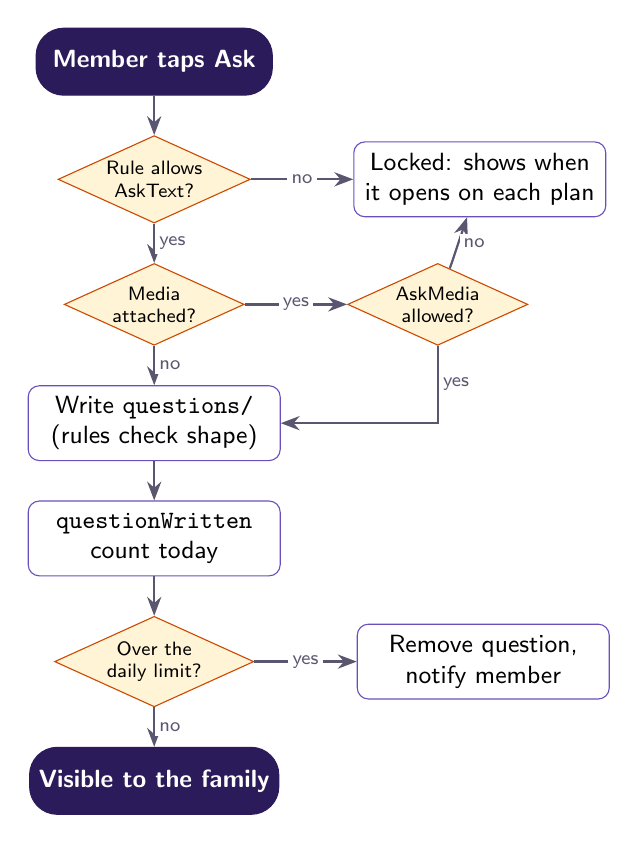
\begin{tikzpicture}[node distance=0.5cm and 1.0cm]
  \node[term] (a) {Member taps Ask};
  \node[dec,below=of a] (r) {Rule allows\\AskText?};
  \node[fstep,right=1.3cm of r] (lock) {Locked: shows when\\it opens on each plan};
  \node[dec,below=of r] (m) {Media\\attached?};
  \node[dec,right=1.3cm of m] (mm) {AskMedia\\allowed?};
  \node[fstep,below=of m] (w) {Write \texttt{questions/}\\(rules check shape)};
  \node[fstep,below=of w] (t) {\texttt{questionWritten}\\count today};
  \node[dec,below=of t] (lim) {Over the\\daily limit?};
  \node[fstep,right=1.3cm of lim] (del) {Remove question,\\notify member};
  \node[term,below=of lim] (ok) {Visible to the family};
  \draw[flow] (a) -- (r); \draw[flow] (r) -- node[lbl]{no} (lock); \draw[flow] (r) -- node[lbl,right]{yes} (m);
  \draw[flow] (m) -- node[lbl]{yes} (mm); \draw[flow] (mm) -- node[lbl,right]{no} (lock);
  \draw[flow] (mm.south) |- node[lbl,pos=0.25,right]{yes} (w.east);
  \draw[flow] (m) -- node[lbl,right]{no} (w); \draw[flow] (w) -- (t); \draw[flow] (t) -- (lim);
  \draw[flow] (lim) -- node[lbl]{yes} (del); \draw[flow] (lim) -- node[lbl,right]{no} (ok);
\end{tikzpicture}
\caption{Q\&A posting with plan rules and the daily limit}
\end{figure}

\section{Personal call (WebRTC)}
\begin{figure}[H]
\centering
\resizebox{\textwidth}{!}{%
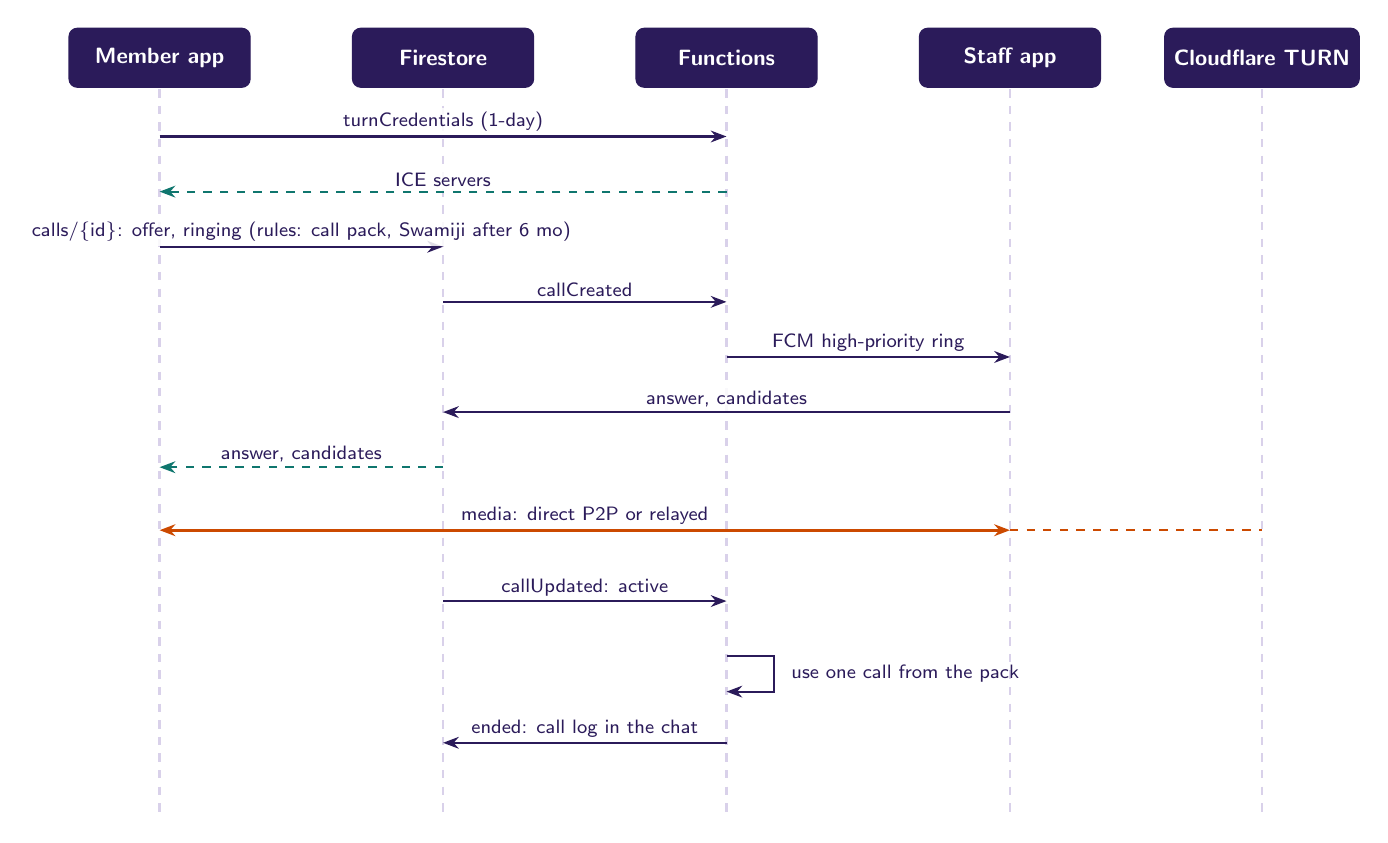
\begin{tikzpicture}
  \foreach \x/\n in {0/Member app,3.6/Firestore,7.2/Functions,10.8/Staff app,14.0/Cloudflare TURN}{
    \node[part] at (\x,0) {\n}; \draw[life] (\x,-0.4) -- (\x,-9.6);}
  \seqmsg{0}{7.2}{-1.0}{turnCredentials (1-day)}
  \seqret{7.2}{0}{-1.7}{ICE servers}
  \seqmsg{0}{3.6}{-2.4}{calls/\{id\}: offer, ringing (rules: call pack, Swamiji after 6 mo)}
  \seqmsg{3.6}{7.2}{-3.1}{callCreated}
  \seqmsg{7.2}{10.8}{-3.8}{FCM high-priority ring}
  \seqmsg{10.8}{3.6}{-4.5}{answer, candidates}
  \seqret{3.6}{0}{-5.2}{answer, candidates}
  \draw[{Stealth[length=2mm]}-{Stealth[length=2mm]},very thick,draw=ojOrange] (0,-6.0) -- node[mlbl]{media: direct P2P or relayed} (10.8,-6.0);
  \draw[thick,ojOrange,dashed] (10.8,-6.0) -- (14.0,-6.0);
  \seqmsg{3.6}{7.2}{-6.9}{callUpdated: active}
  \seqself{7.2}{-7.6}{use one call from the pack}
  \seqmsg{7.2}{3.6}{-8.7}{ended: call log in the chat}
\end{tikzpicture}}
\caption{Call set-up, signalling and billing of a call}
\end{figure}

\section{Thought of the Day at 4 am local time}
\begin{figure}[H]
\centering
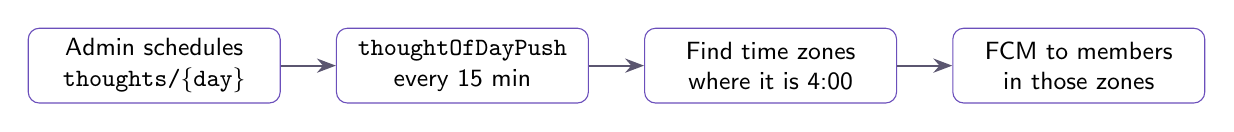
\begin{tikzpicture}[node distance=0.4cm and 0.7cm]
  \node[fstep] (a) {Admin schedules\\\texttt{thoughts/\{day\}}};
  \node[fstep,right=of a] (b) {\texttt{thoughtOfDayPush}\\every 15 min};
  \node[fstep,right=of b] (c) {Find time zones\\where it is 4:00};
  \node[fstep,right=of c] (d) {FCM to members\\in those zones};
  \draw[flow] (a) -- (b); \draw[flow] (b) -- (c); \draw[flow] (c) -- (d);
\end{tikzpicture}
\caption{Daily Thought push by time zone}
\end{figure}

% =====================================================================
\chapter{Security architecture}

\begin{figure}[H]
\centering
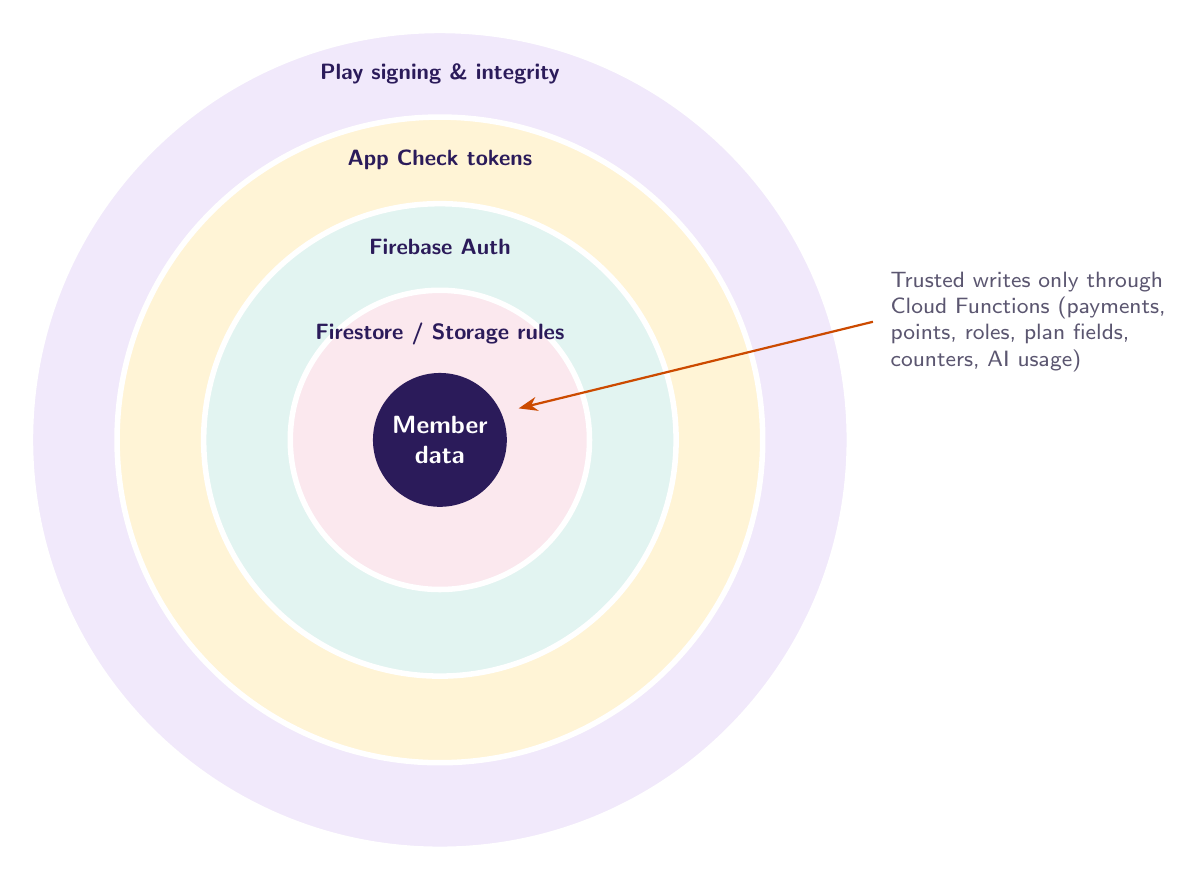
\begin{tikzpicture}
  \foreach \r/\c/\t/\a in {5.2/ojLav/Google Play \& device integrity/90, 4.1/ojGoldL/App Check (Play Integrity)/90, 3.0/ojTealL/Firebase Auth identity/90, 1.9/ojRose/Security rules per document/90}{
    \fill[\c,draw=white,line width=2pt] (0,0) circle (\r);}
  \fill[ojDeep] (0,0) circle (0.85);
  \node[text=white,font=\bfseries\small,align=center] at (0,0) {Member\\data};
  \node[font=\footnotesize\bfseries,text=ojDeep] at (0,4.65) {Play signing \& integrity};
  \node[font=\footnotesize\bfseries,text=ojDeep] at (0,3.55) {App Check tokens};
  \node[font=\footnotesize\bfseries,text=ojDeep] at (0,2.45) {Firebase Auth};
  \node[font=\footnotesize\bfseries,text=ojDeep] at (0,1.35) {Firestore / Storage rules};
  \node[font=\footnotesize,text=ojGrey,align=left,anchor=west] at (5.6,1.5) {Trusted writes only through\\Cloud Functions (payments,\\points, roles, plan fields,\\counters, AI usage)};
  \draw[flowO] (5.5,1.5) -- (1.0,0.4);
\end{tikzpicture}
\caption{Defence in depth}
\end{figure}

\begin{tabularx}{\textwidth}{@{}p{3.6cm}L@{}}
\headrow \thead{Threat} & \thead{Control} \\
Modified app grants itself Gold & Plan fields and entitlements are function-only; rules read them server-side. \\
Replayed or shared purchase & Token claimed by its SHA-256 for one account; product id must match the token; acknowledged server-side. \\
Replaced subscription cancels new plan & Entitlement keeps \texttt{tokenKey}; notices for other tokens are ignored. \\
Bots and scripted clients & App Check with Play Integrity, enforced on AI and sensitive callables. \\
AI key leakage & NVIDIA key in Secret Manager; only \texttt{askSwamiji} can read it. \\
TURN abuse & Cloudflare credentials issued per user, valid 24 h; key in \texttt{serverConfig} (no client rule). \\
Spam and links & Links in posts go to moderation (\texttt{status: pending}); daily Q\&A limit; reports queue. \\
Privacy & Birth date never public; \texttt{publicProfiles} mirror exposes month only; Gold can hide profile. \\
Over-sized uploads & Storage rules check type and size for chat, Q\&A and photos. \\
\bottomrule
\end{tabularx}

% =====================================================================
\chapter{Deployment and operations}

\section{Environments}
\begin{tabularx}{\textwidth}{@{}p{2.8cm}p{3.6cm}L@{}}
\headrow \thead{Environment} & \thead{Project} & \thead{Use} \\
Local & \texttt{demo-ojas} (emulators) & Auth, Firestore, Storage and Functions emulators; debug app via \texttt{debug.ojas.emulator}; rules and function tests. \\
Production & \texttt{ojas-family-app} & asia-south1; deployed by the owner with the Firebase CLI. \\
\bottomrule
\end{tabularx}

\section{Release pipeline}
\begin{figure}[H]
\centering
\resizebox{\textwidth}{!}{%
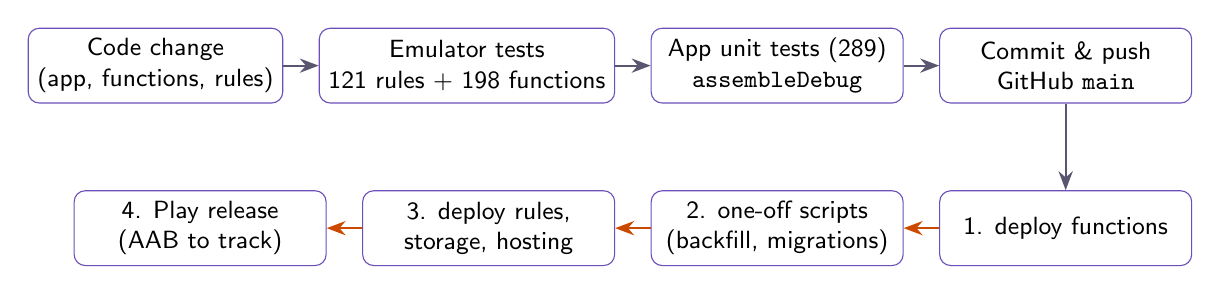
\begin{tikzpicture}[node distance=0.45cm]
  \node[fstep] (a) {Code change\\(app, functions, rules)};
  \node[fstep,right=of a] (b) {Emulator tests\\121 rules + 198 functions};
  \node[fstep,right=of b] (c) {App unit tests (289)\\\texttt{assembleDebug}};
  \node[fstep,right=of c] (d) {Commit \& push\\GitHub \texttt{main}};
  \node[fstep,below=1.1cm of d] (e) {1. deploy functions};
  \node[fstep,left=of e] (f) {2. one-off scripts\\(backfill, migrations)};
  \node[fstep,left=of f] (g) {3. deploy rules,\\storage, hosting};
  \node[fstep,left=of g] (h) {4. Play release\\(AAB to track)};
  \draw[flow] (a) -- (b); \draw[flow] (b) -- (c); \draw[flow] (c) -- (d); \draw[flow] (d) -- (e);
  \draw[flowO] (e) -- (f); \draw[flowO] (f) -- (g); \draw[flowO] (g) -- (h);
\end{tikzpicture}}
\caption{Build, test and deploy order}
\end{figure}

\begin{riskbox}[Deploy order matters]
Rules that read new fields must go out \emph{after} the functions and scripts that write them. On 20 November the three commands were run as one, and the rules went live a few minutes before the backfill; run each command on its own and wait for it to finish.
\end{riskbox}

\section{Monitoring}
\begin{itemize}
  \item Crashlytics and Analytics in the app; Cloud Logging for functions.
  \item \texttt{dailyStats} feeds the admin dashboard: active members, plans, languages, countries.
  \item Play Console vitals for ANRs and crashes; Play RTDN keeps subscriptions in step.
\end{itemize}

% =====================================================================
\chapter{Quality and testing}

\begin{figure}[H]
\centering
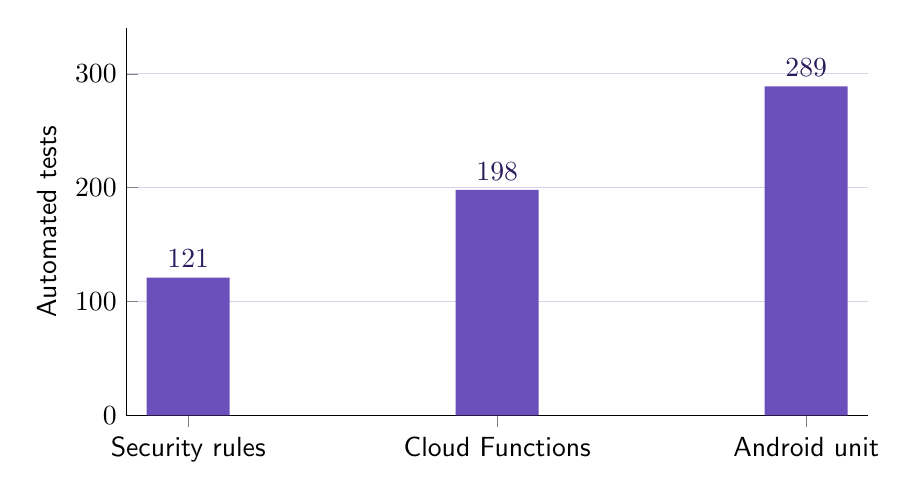
\begin{tikzpicture}
\begin{axis}[
  ybar, width=11cm, height=6.5cm, bar width=30pt, ymin=0, ymax=340,
  symbolic x coords={Security rules,Cloud Functions,Android unit},
  xtick=data, ylabel={Automated tests}, nodes near coords,
  nodes near coords style={font=\bfseries,color=ojDeep},
  axis x line*=bottom, axis y line*=left, ymajorgrids, major grid style={ojLine}]
\addplot[fill=ojPurple,draw=none] coordinates {(Security rules,121) (Cloud Functions,198) (Android unit,289)};
\end{axis}
\end{tikzpicture}
\caption{Automated tests by layer (608 in total, all passing on 20 Nov 2026)}
\end{figure}

\begin{figure}[H]
\centering
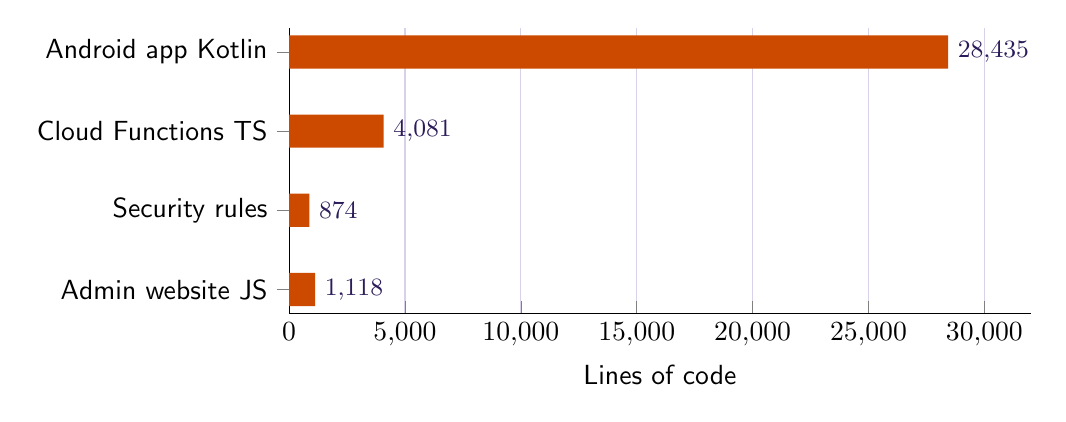
\begin{tikzpicture}
\begin{axis}[
  xbar, width=11cm, height=5.2cm, bar width=12pt, xmin=0, xmax=32000,
  symbolic y coords={Admin website JS,Security rules,Cloud Functions TS,Android app Kotlin},
  ytick=data, xlabel={Lines of code}, nodes near coords,
  nodes near coords style={font=\small\bfseries,color=ojDeep},
  scaled x ticks=false, xticklabel style={/pgf/number format/fixed},
  axis x line*=bottom, axis y line*=left, xmajorgrids, major grid style={ojLine}]
\addplot[fill=ojOrange,draw=none] coordinates {(1118,Admin website JS) (874,Security rules) (4081,Cloud Functions TS) (28435,Android app Kotlin)};
\end{axis}
\end{tikzpicture}
\caption{Code size by component}
\end{figure}

\begin{tabularx}{\textwidth}{@{}p{3.4cm}L@{}}
\headrow \thead{Suite} & \thead{What it proves} \\
Rules (emulator) & Each plan, role and stage can and cannot read or write each collection; chat and calls by channel. \\
Functions (emulator) & Purchases, upgrade notices, limits, points, counters, AI quota, call credits, link previews. \\
Android unit & Plan table, permissions, lock texts, view models, content access, formatting. \\
\bottomrule
\end{tabularx}

% =====================================================================
\chapter{Application screens}
\label{chap:screens}
Taken on an Android emulator against the local backend with sample data (no production data).

\newcommand{\shot}[2]{\begin{subfigure}[t]{0.23\textwidth}\centering\includegraphics[width=\linewidth]{images/#1}\caption{#2}\end{subfigure}}

\begin{figure}[H]
\centering
\shot{01-welcome.png}{Language}\hfill
\shot{02-signin.png}{Sign-in}\hfill
\shot{03-profile.png}{Onboarding}\hfill
\shot{04-points.png}{Daily point}
\caption{First run}
\end{figure}

\begin{figure}[H]
\centering
\shot{05-home.png}{Home}\hfill
\shot{13-announcements.png}{Announcements}\hfill
\shot{07-practice.png}{Practice}\hfill
\shot{08-ask.png}{Ask}
\caption{Main tabs}
\end{figure}

\begin{figure}[H]
\centering
\shot{12-ai.png}{Ask Swamiji AI}\hfill
\shot{06-community.png}{Daily Activity}\hfill
\shot{09-profile.png}{Profile}\hfill
\shot{14-admin-tools.png}{Admin tools}
\caption{AI, community, profile and administration}
\end{figure}

% =====================================================================
\chapter{Risks and roadmap}

\section{Risks}
\begin{tabularx}{\textwidth}{@{}p{4.6cm}cL@{}}
\headrow \thead{Risk} & \thead{Level} & \thead{Mitigation} \\
Gold product not yet in Play Console & \textcolor{ojOrange}{\bfseries High} & Create \texttt{membership\_gold\_monthly} (Rs.\,101) before release. \\
Older app versions show buttons the rules refuse & Medium & Ask members to update; consider a minimum-version check. \\
Plan table drift between three copies & Medium & Tests in each layer; change all three in one commit. \\
NVIDIA API outage & Medium & One retry; clear error message; AI is not on the critical path. \\
Single-owner deploys & Low & Written deploy order; one command at a time. \\
Profile still shows the old member-level ladder & Low & Replace with the plan card in a follow-up. \\
\bottomrule
\end{tabularx}

\section{Roadmap}
\begin{figure}[H]
\centering
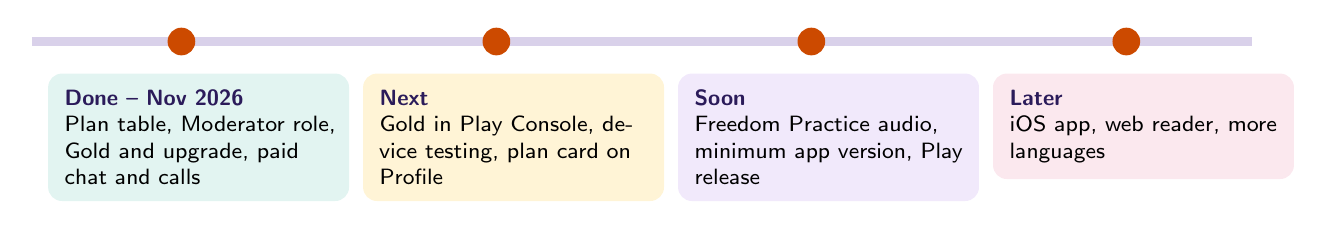
\begin{tikzpicture}[ms/.style={draw=none,fill=#1,rounded corners=5pt,text width=3.4cm,align=left,font=\footnotesize,inner sep=6pt}]
  \draw[line width=3pt,ojLine] (0,0) -- (15.5,0);
  \fill[ojOrange] (1.9,0) circle (5pt);
  \node[ms=ojTealL,anchor=north west] at (0.2,-0.4) {{\bfseries\color{ojDeep}Done \textendash\ Nov 2026}\\Plan table, Moderator role, Gold and upgrade, paid chat and calls};
  \fill[ojOrange] (5.9,0) circle (5pt);
  \node[ms=ojGoldL,anchor=north west] at (4.2,-0.4) {{\bfseries\color{ojDeep}Next}\\Gold in Play Console, device testing, plan card on Profile};
  \fill[ojOrange] (9.9,0) circle (5pt);
  \node[ms=ojLav,anchor=north west] at (8.2,-0.4) {{\bfseries\color{ojDeep}Soon}\\Freedom Practice audio, minimum app version, Play release};
  \fill[ojOrange] (13.9,0) circle (5pt);
  \node[ms=ojRose,anchor=north west] at (12.2,-0.4) {{\bfseries\color{ojDeep}Later}\\iOS app, web reader, more languages};
\end{tikzpicture}
\caption{Roadmap}
\end{figure}

% =====================================================================
\appendix
\chapter{Glossary}
\begin{tabularx}{\textwidth}{@{}p{3.4cm}L@{}}
\headrow \thead{Term} & \thead{Meaning} \\
Stage & Days since joining (Free) or since the paid plan began (Silver, Gold). \\
Entitlement & A paid access record: membership, chat or call, with an expiry. \\
RTDN & Real-time developer notifications from Google Play about subscriptions. \\
App Check & Firebase proof that a request comes from the genuine app on a genuine device. \\
TURN & A relay server that carries call media when phones cannot connect directly. \\
RAG & Retrieval-augmented generation: the AI answers from retrieved passages of Swamiji's teachings. \\
Freedom Points & In-app points earned by daily presence, practice and profile completion. \\
\bottomrule
\end{tabularx}

\end{document}
